\section{Geometries}\label{sec:Geometries}

%% The vertex detector is responsible for the identification of the heavy quarks. The CLIC experimental conditions push the technology of the vertex detector to its limits as it needs to have high spatial resolution, precise timing capabilities, full geometrical space coverage for low polar angles $\theta$, low mass and sufficient heat removal from sensors and readout. The size of the pixels for the CLIC vertex detector is much smaller than the pixels used at the hadron colliders, while complex on-chip readout and ultra-thin materials are needed. In addition, the vertex detectors are located very close to the interaction point where the beam-induced background rates are very high. Several R\&D programs are addressing the various challenges such as sensors, readout, interconnects, power pulsing, thin supports and air cooling. \\
%% This note focuses on the CLIC\_SiD vertex geometry as described in \cite{CLICCDR2012}. This geometry is referred as CLIC\_SiD\_CDR in this note. It is used as a starting point for the implementation of new geometries. The new suggested geometries are conceived by varying the CLIC\_SiD\_CDR geometry. Three new geometries are studied: the first one contains a spiral arrangement of sensors in the vertex endcap instead of disks and the second one contains double-layered sensors in the vertex barrel and in the spiral vertex endcap. A third variation is used to get closer to a more realistic model with higher material budget which takes into account the mechanical support, the electronics used for the readout and the power pulsing of the pixels.
% The vertex detector is responsible for the identification of the heavy quarks. In CLIC, the vertex detector needs to have very low material budget to minimize multiple scatterings of the particles in the material to achieve more precise measurements. For this purpose, the non-sensitive material used for example for the mechanical support or the heat removal is wished to be minimized. Airflow cooling is aimed to be used as the heat removal technique for the pixel sensors. Also, double-layered sensors with higher number of detecting material increase the precision of the measurements. \\
The starting point for the studies described in this note is the CLIC\_SiD vertex geometry as described in the CDR~\cite{CLICCDR2012}. This geometry is referred to as the CDR geometry in the following. \\
Three new geometries are implemented as variations to the CDR layout. The first geometry contains a spiral arrangement of sensors in the vertex endcaps (Section~\ref{sec:CLIC_SiD_spirals}). The second geometry, in addition to a spiral arrangement of the sensors in the endcap regions, uses double-layered modules for the whole vertex detector (Section~\ref{sec:CLIC_SiD_double_spirals}). A third variation with twice the material budget has been used, which takes into account the mechanical support, the readout electronics and the cables (Section~\ref{sec:CLIC_SiD_double_spirals_heavy}).

\subsection{Coordinate system}
The right-handed coordinate system in which the detector is described is shown in Figure~\ref{fig:coord_system}. The beam axis is parallel to the z-axis. The polar angle $\theta$ is the angle between the z-axis and the radial coordinate r, and $\phi$ is the azimuthal angle.
\begin{figure}[H]
  \centering
  % \begin{tikzpicture}
  %   \node[anchor=south west,inner sep=0] (image) at (0,0){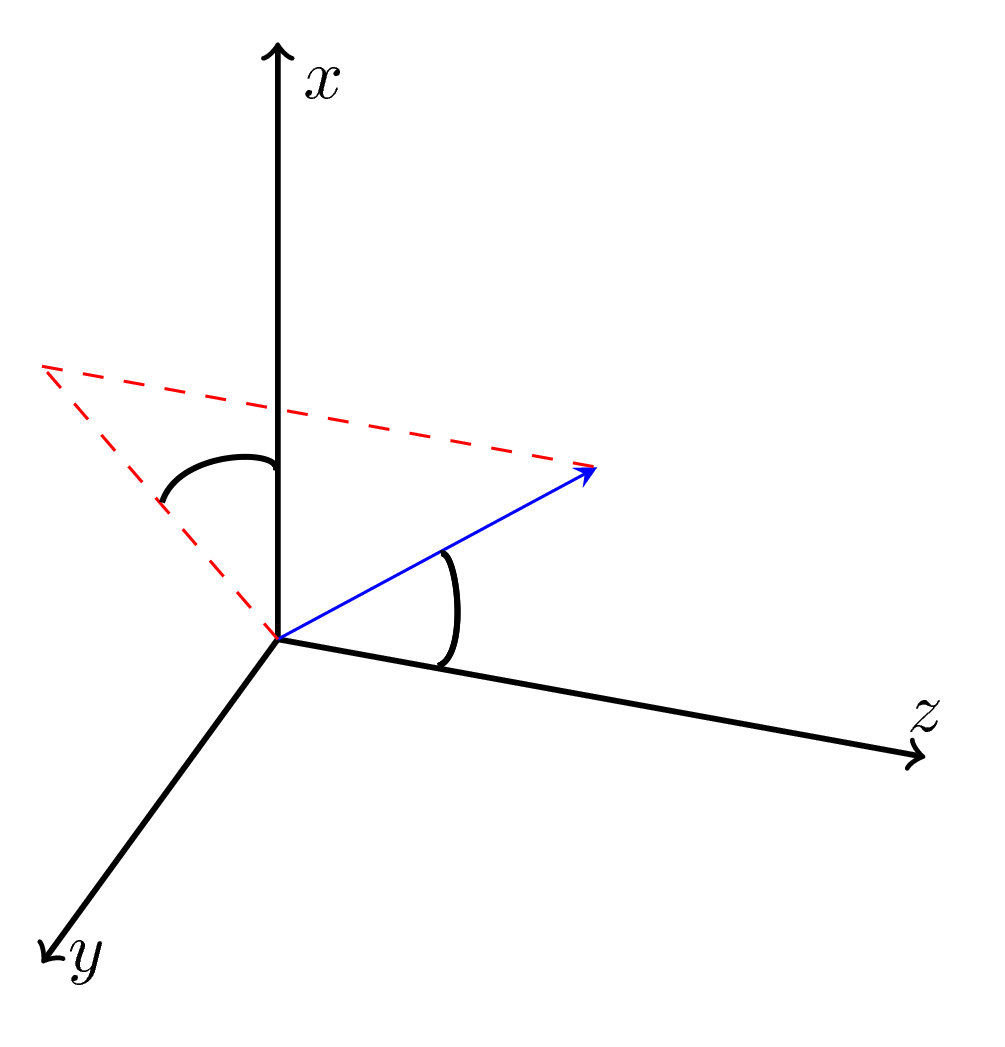
\includegraphics[width=0.2\textheight]{Figures/Geometries/coordinates.png}};
  %   \begin{scope}[x={(image.south east)},y={(image.north west)}]
  %     \node[left, text=black] at (0.27, 0.6){$\phi$};
  %     \node[right, text=black] at (0.45, 0.45){$\theta$};
  %   \end{scope}
  % \end{tikzpicture}
  \tdplotsetmaincoords{60}{120}
  \begin{tikzpicture}
    [scale=3,
      tdplot_main_coords,
      axis/.style={->,black,thick},
      vector/.style={-stealth,ForestGreen,very thick},
      vector guide/.style={dashed,ForestGreen,thick},
      angle/.style={ForestGreen,thick}]
    
    % standard tikz coordinate definition using x, y, z coords
    \coordinate (O) at (0,0,0);
    
    % tikz-3dplot coordinate definition using r, theta, phi coords
    \tdplotsetcoord{P}{.8}{55}{60}
    
    % draw axes
    \draw[axis] (0,0,0) -- (1,0,0) node[anchor=north east]{$x$};
    \draw[axis] (0,0,0) -- (0,1,0) node[anchor=north west]{$y$};
    \draw[axis] (0,0,0) -- (0,0,1) node[anchor=south]{$z$};
    
    % draw a vector from O to P
    \draw[vector] (O) -- (P);
    
    % draw guide lines to components
    \draw[vector guide] (O) -- (Pxy);
    \draw[vector guide] (Pxy) -- (P);
    
    % draw an arc illustrating the angle defining the orientation
    \tdplotdrawarc[angle]{(O)}{.35}{0}{60}{anchor=north}{$\phi$}
    
    % define the rotated coordinate frame to lie in the "theta plane"
    \tdplotsetthetaplanecoords{55}
    
    \tdplotdrawarc[tdplot_rotated_coords,angle]{(O)}{.35}{0}{55}
                  {anchor=south west}{$\theta$}
                  
  \end{tikzpicture}
  \caption{The right-handed coordinate system used to describe the geometry where the beam axis is parallel to the z-axis.}
  \label{fig:coord_system}
\end{figure}
%% \begin{figure}[H]
%%   \centering
%%   % \begin{tikzpicture}
%%   %   \node[anchor=south west,inner sep=0] (image) at (0,0){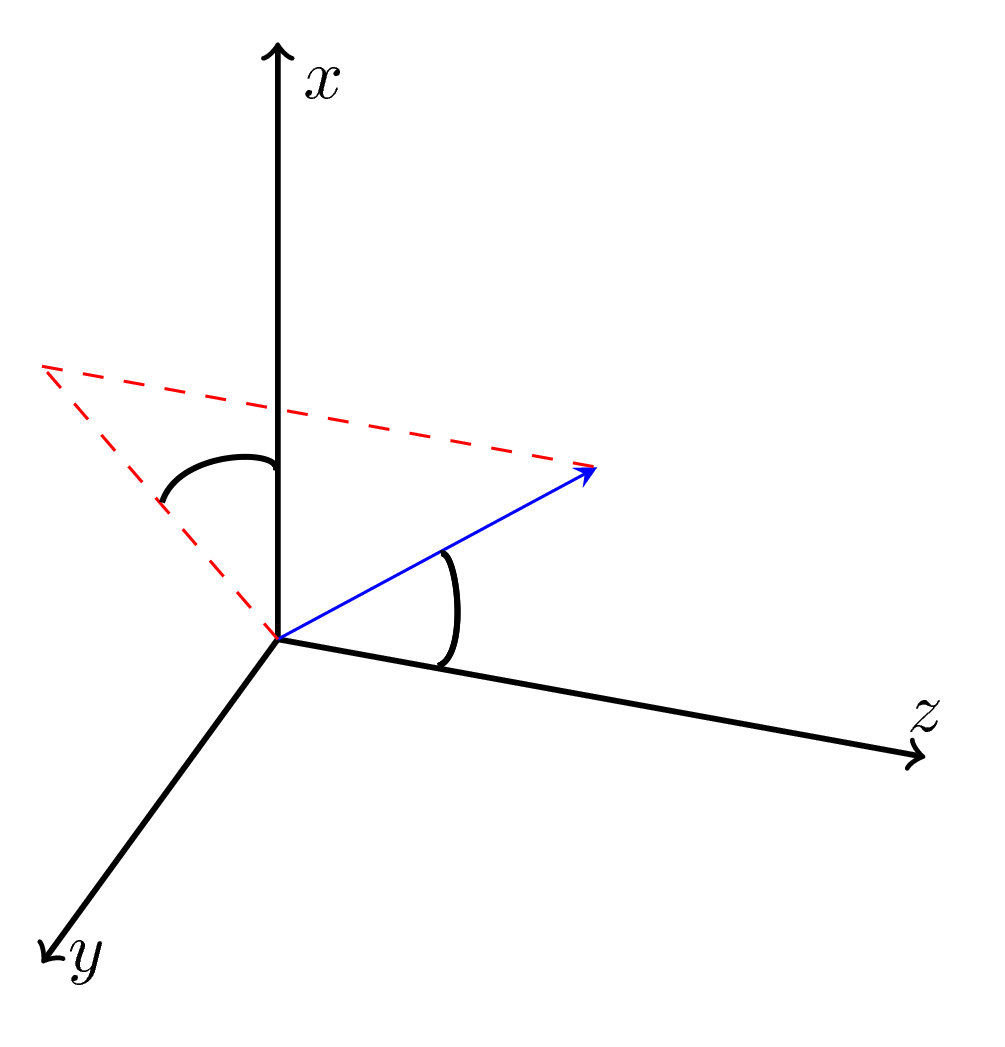
\includegraphics[width=0.2\textheight]{Figures/Geometries/coordinates.png}};
%%   %   \begin{scope}[x={(image.south east)},y={(image.north west)}]
%%   %     \node[left, text=black] at (0.27, 0.6){$\phi$};
%%   %     \node[right, text=black] at (0.45, 0.45){$\theta$};
%%   %   \end{scope}
%%   % \end{tikzpicture}
%%   \begin{tikzpicture}
%%     \node[anchor=south west,inner sep=0] (image) at (0, 0){\includegraphics[trim=80mm 200mm 80mm 50mm, clip, angle=286, width=0.3\textheight]{coord.pdf}};  
%%     \node[] at (2.4, 0.4) {$y$}; 
%%     \node[] at (0.4, 5) {$x$};
%%     \node[] at (5.5, 4.4) {$z$};
%%     \node[color=ForestGreen] at (3.5, 3.5) {$\theta$};
%%     \node[color=ForestGreen] at (1.8, 3.5) {$\phi$};
%%   \end{tikzpicture}
%%   \caption{The coordinate system in which the detector is defined. The beam line is parallel to the z-axis.}
%%   \label{fig:coord_system}
%% \end{figure}
%% \begin{figure}[H]
%%   \centering
%%   % \begin{tikzpicture}
%%   %   \node[anchor=south west,inner sep=0] (image) at (0,0){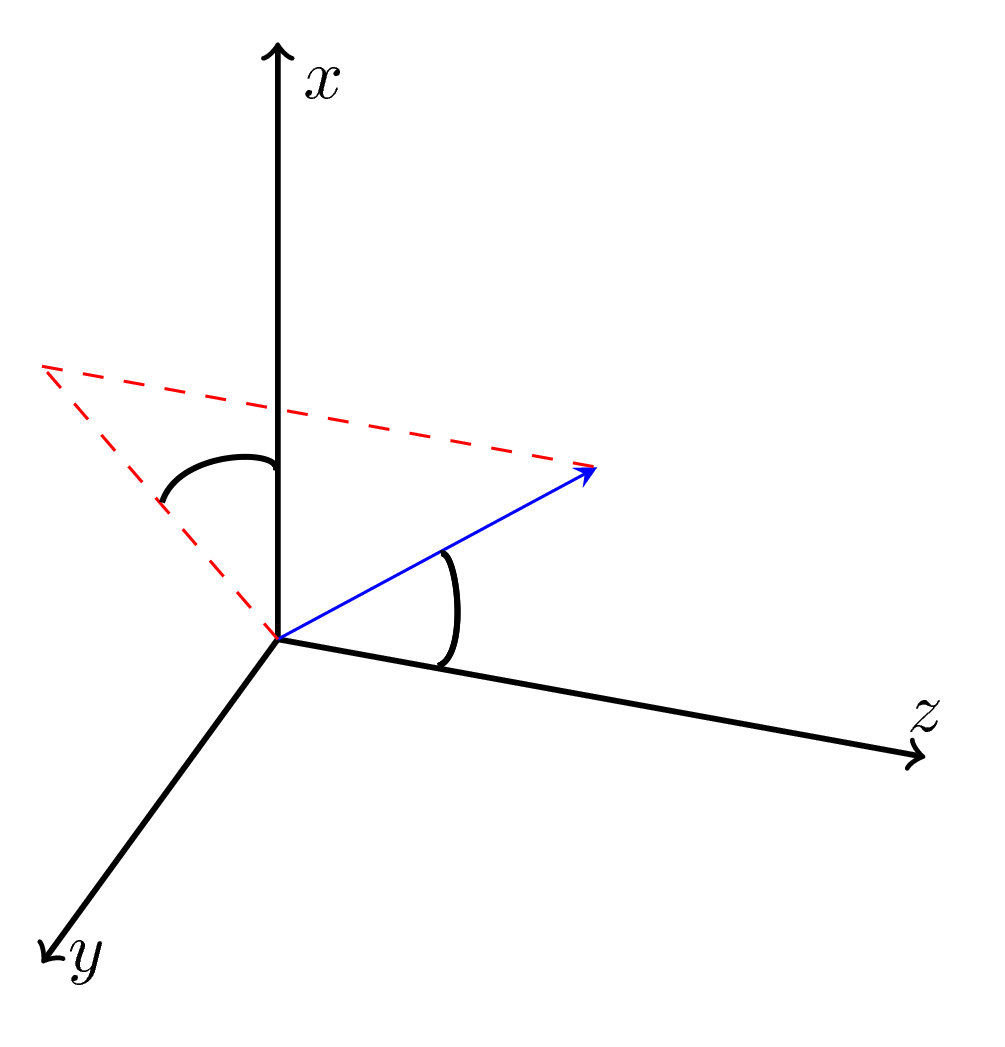
\includegraphics[width=0.2\textheight]{Figures/Geometries/coordinates.png}};
%%   %   \begin{scope}[x={(image.south east)},y={(image.north west)}]
%%   %     \node[left, text=black] at (0.27, 0.6){$\phi$};
%%   %     \node[right, text=black] at (0.45, 0.45){$\theta$};
%%   %   \end{scope}
%%   % \end{tikzpicture}
%%   %% \begin{tikzpicture}
%%   %%   \node[anchor=south west,inner sep=0] (image) at (0, 0){\includegraphics[trim=80mm 200mm 80mm 50mm, clip, angle=286, width=0.3\textheight]{coord.pdf}};  
%%   %%   \node[] at (2.4, 0.4) {$y$}; 
%%   %%   \node[] at (0.4, 5) {$x$};
%%   %%   \node[] at (5.5, 4.4) {$z$};
%%   %%   \node[color=ForestGreen] at (3.5, 3.5) {$\theta$};
%%   %%   \node[color=ForestGreen] at (1.8, 3.5) {$\phi$};
%%   %% \end{tikzpicture}
%%   \caption{The coordinate system in which the detector is defined. The beam line is parallel to the z-axis.}
%%   \label{fig:coord_system}
%% \end{figure}
%----------------------------------------------------------------------
\subsection{The CDR geometry}\label{sec:CLIC_SiD_CDR}
The term "CDR geometry" refers to the CLIC\_SiD geometry as defined in~\cite{CLICCDR2012}. It consists of five concentric layers in the vertex barrel (cf. Figure~\ref{fig:vertex_barrel}) and four disks in the vertex endcaps. 

\begin{figure}[H]
  \centering
  \begin{tikzpicture}
    \node[anchor=south west,inner sep=0] (image) at (0, 0){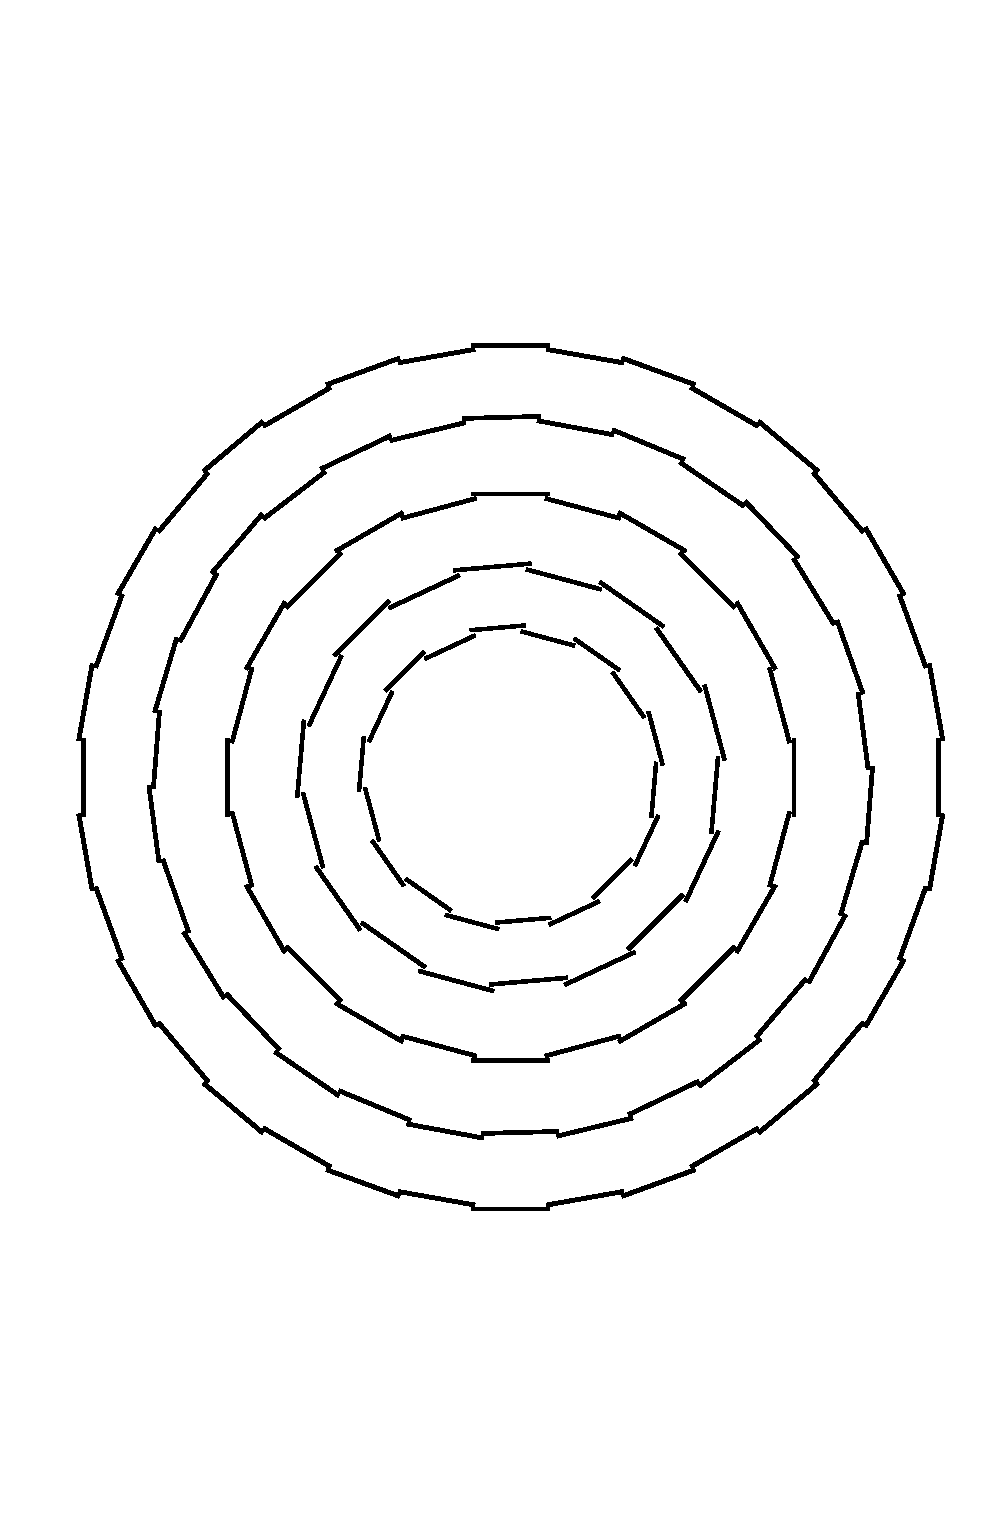
\includegraphics[trim = 0mm 30mm 0mm 30mm, clip,  width=0.3\textheight]{Figures/Geometries/default_barrel.pdf}};
    \draw[->,line width=.4pt, color=ForestGreen](3.6, 4) -- (7.1, 4);
    \node[right, color=ForestGreen] at (7.1, 4) {$x$};
    \draw[->,line width=.4pt, color=ForestGreen](3.6, 4) -- (3.6, 7.5);
    \node[right, color=ForestGreen] at (3.6, 7.5) {$y$};
  \end{tikzpicture}
  \label{fig:vertex_barrel_b}
  \caption{Schematic layout of the vertex barrel detector in the xy-plane for the CDR geometry.}\label{fig:vertex_barrel}
\end{figure}


%% \begin{figure}[H]
%%   \centering
%%   \begin{subfigure}[H]{0.2\textwidth}
%%     \hspace{-5cm}
%%     \vspace{1cm}
%%     \includegraphics[page=5, trim=0mm 155mm 100mm 50mm, clip, width=0.3\textheight]{Figures/Geometries/LCD-2011-009.pdf}
%%     \caption{}
%%     \label{fig:vertex_barrel_a}
%%   \end{subfigure} \quad
%%   \begin{subfigure}[H]{0.2\textwidth}
%%     \hspace{3cm}
%%     \begin{tikzpicture}
%%       \node[anchor=south west,inner sep=0] (image) at (0, 0){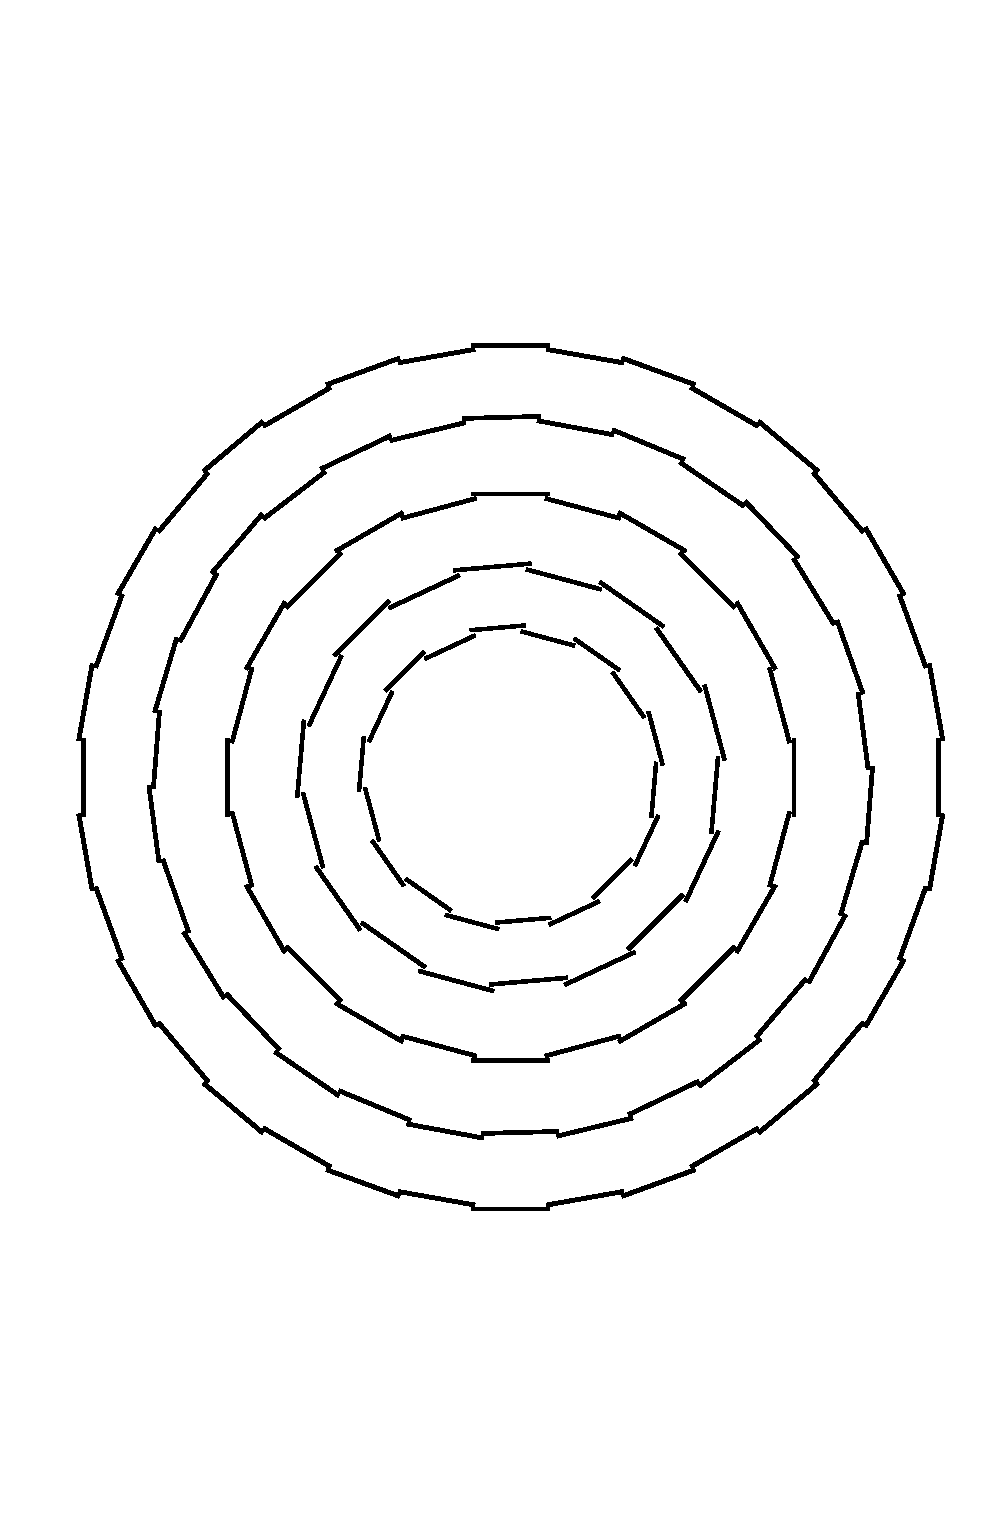
\includegraphics[trim = 0mm 30mm 0mm 30mm, clip,  width=0.3\textheight]{Figures/Geometries/default_barrel.pdf}};
%%       \draw[->,line width=.4pt, color=ForestGreen](3.2, 3.5) -- (6.5, 3.5);
%%       \node[right, color=ForestGreen] at (6.5, 3.5) {$x$};
%%       \draw[->,line width=.4pt, color=ForestGreen](3.2, 3.5) -- (3.2, 6.8);
%%       \node[right, color=ForestGreen] at (3.2, 6.8) {$y$};
%%     \end{tikzpicture}
%%     \caption{}
%%     \label{fig:vertex_barrel_b}
%%   \end{subfigure}
%%   \caption{Schematic layout of the vertex barrel detector in the xy-plane for the CDR geometry. The distances in (a) are given in mm. From~\cite{Grefe2011}.}\label{fig:vertex_barrel}
%% \end{figure}


Each layer in the barrel is composed of several modules as listed in Table~\ref{tab:params_default}. Each module contains a silicon sensor with a thickness of \SI{50}{\micro\meter}. The silicon sensor is the sensitive part of the module which detects the particles passing through it. It is followed by a layer of carbon fiber with a thickness of \SI{130}{\micro\meter}, emulating the material for readout, cabling and supports. The total amount of material per layer corresponds to $0.11\%X_{0}$.\\
 
\begin{table}[H]
  \caption{Parameters for the vertex detector barrel layers for the CDR geometry. \textit{N} represents the number of modules in a layer, \textit{r} the mean radius of the layer, \textit{z} the half-length and \textit{w} the width of the module. In the \textsc{Geant4} simulations, each module consists of \SI{50}{\micro\meter} of silicon followed by \SI{130}{\micro\meter} of carbon fiber. From~\cite{Grefe2011}.}
  \begin{center}
    \begin{tabular}{ c c c c c }
      \hline
      Layer & N & r[mm] & z[mm] & w[mm]\\ \hline \hline
      1 & 18 & 27.0 & 98.5 & 9.8 \\ \hline
      2 & 18 & 38.0 & 98.5 & 13.8 \\ \hline
      3 & 24 & 51.0 & 98.5 & 13.8 \\ \hline
      4 & 30 & 64.0 & 98.5 & 13.8 \\ \hline
      5 & 36 & 77.0 & 98.5 & 13.8 \\ \hline
    \end{tabular}
  \end{center}
  \label{tab:params_default}
\end{table}

The vertex detector contains 4 disks in the endcap regions made of silicon pixel detectors with the parameters given in Table~\ref{tab:params_default_endcap}. Figure~\ref{fig:endcap_placement} shows a schematic layout of the vertex detector with highlighted vertex barrel and endcap. The vertex detector is surrounded by the main tracking system made of silicon strip detectors. 
\begin{figure}[H]
  %\centering
  \hspace{-2cm}
  \begin{tikzpicture}
    \node[anchor=south west,inner sep=0] (image) at (0,0){\includegraphics[page=6, trim=0mm 210mm 10mm 40mm, clip, width=0.8\textheight]{Figures/Geometries/LCD-2011-009.pdf}};
    \begin{scope}[x={(image.south east)},y={(image.north west)}]
      \draw[Green,ultra thick,rounded corners] (0.15,0.2) rectangle (0.29,0.45);
      \node[above, text=Green] at (0.2, 0.45){Vertex Barrel};
      \draw[Red,ultra thick,rounded corners] (0.295,0.2) rectangle (0.4,0.55);
      \node[above, text=Red] at (0.33, 0.55){Vertex Endcap};
      \draw[->,line width=.4pt, color=ForestGreen](0.9, 0.16) -- (0.95, 0.16);
      \node[right, color=ForestGreen] at (0.95, 0.16) {$z$};
      \draw[->,line width=.4pt, color=ForestGreen](0.9, 0.16) -- (0.9, 0.4);
      \node[right, color=ForestGreen] at (0.9, 0.4) {$y$};
    \end{scope}
  \end{tikzpicture}
  \caption{Schematic layout of the vertex detector in the zy-plane. The distances are given in~mm. From~\cite{Grefe2011}.}
  \label{fig:endcap_placement}
\end{figure}


\begin{table}[H]
  \caption{Parameters for the trapezoidal modules in the forward region
    of the CDR geometry, where \textit{N} represents the number of modules
    in a disk, $r_{in}$ and $r_{out}$ the inner and the outer radius
    for the disks at the outer edge of the trapezoidal modules, $w_{in}$ and $w_{out}$ the inner and the outer
    widths and \textit{z} the position of the modules. In the \textsc{Geant4} simulations, each
    module is made of \SI{50}{\micro\meter} of silicon followed by
    \SI{130}{\micro\meter} of carbon fiber. From~\cite{Grefe2011}.}
  \begin{center}
    \begin{tabular}{ c c c c c c c }
      \hline
      Disk & N & r$_{in}$[mm] & r$_{out}$[mm] & w$_{in}$[mm] & w$_{out}$[mm] & z[mm] \\ \hline \hline
      1 & 16 & 27.0 & 115.0 & 10.8 & 45.1 & 120.0 \\ \hline
      2 & 16 & 27.0 & 115.0 & 10.8 & 45.1 & 160.0 \\ \hline
      3 & 16 & 27.0 & 115.0 & 10.8 & 45.1 & 200.0 \\ \hline
      4 & 16 & 28.1 & 115.0 & 11.3 & 45.1 & 240.0\\ \hline
    \end{tabular}
  \end{center}
  \label{tab:params_default_endcap}
\end{table}

%% The vertex detector is designed to provide excellent point resolution with low material budget in order to minimize multiple scattering in the detector. 
Figure~\ref{fig:default_nb_barrel_endcap} shows the angular coverage of the vertex barrel and the vertex endcaps separately. The vertex detector can measure tracks down to a polar angle of about $\theta = 8^\circ$. The number of measured points affects the performance of the particle track reconstruction. 

\begin{figure}[H]
  \centering
  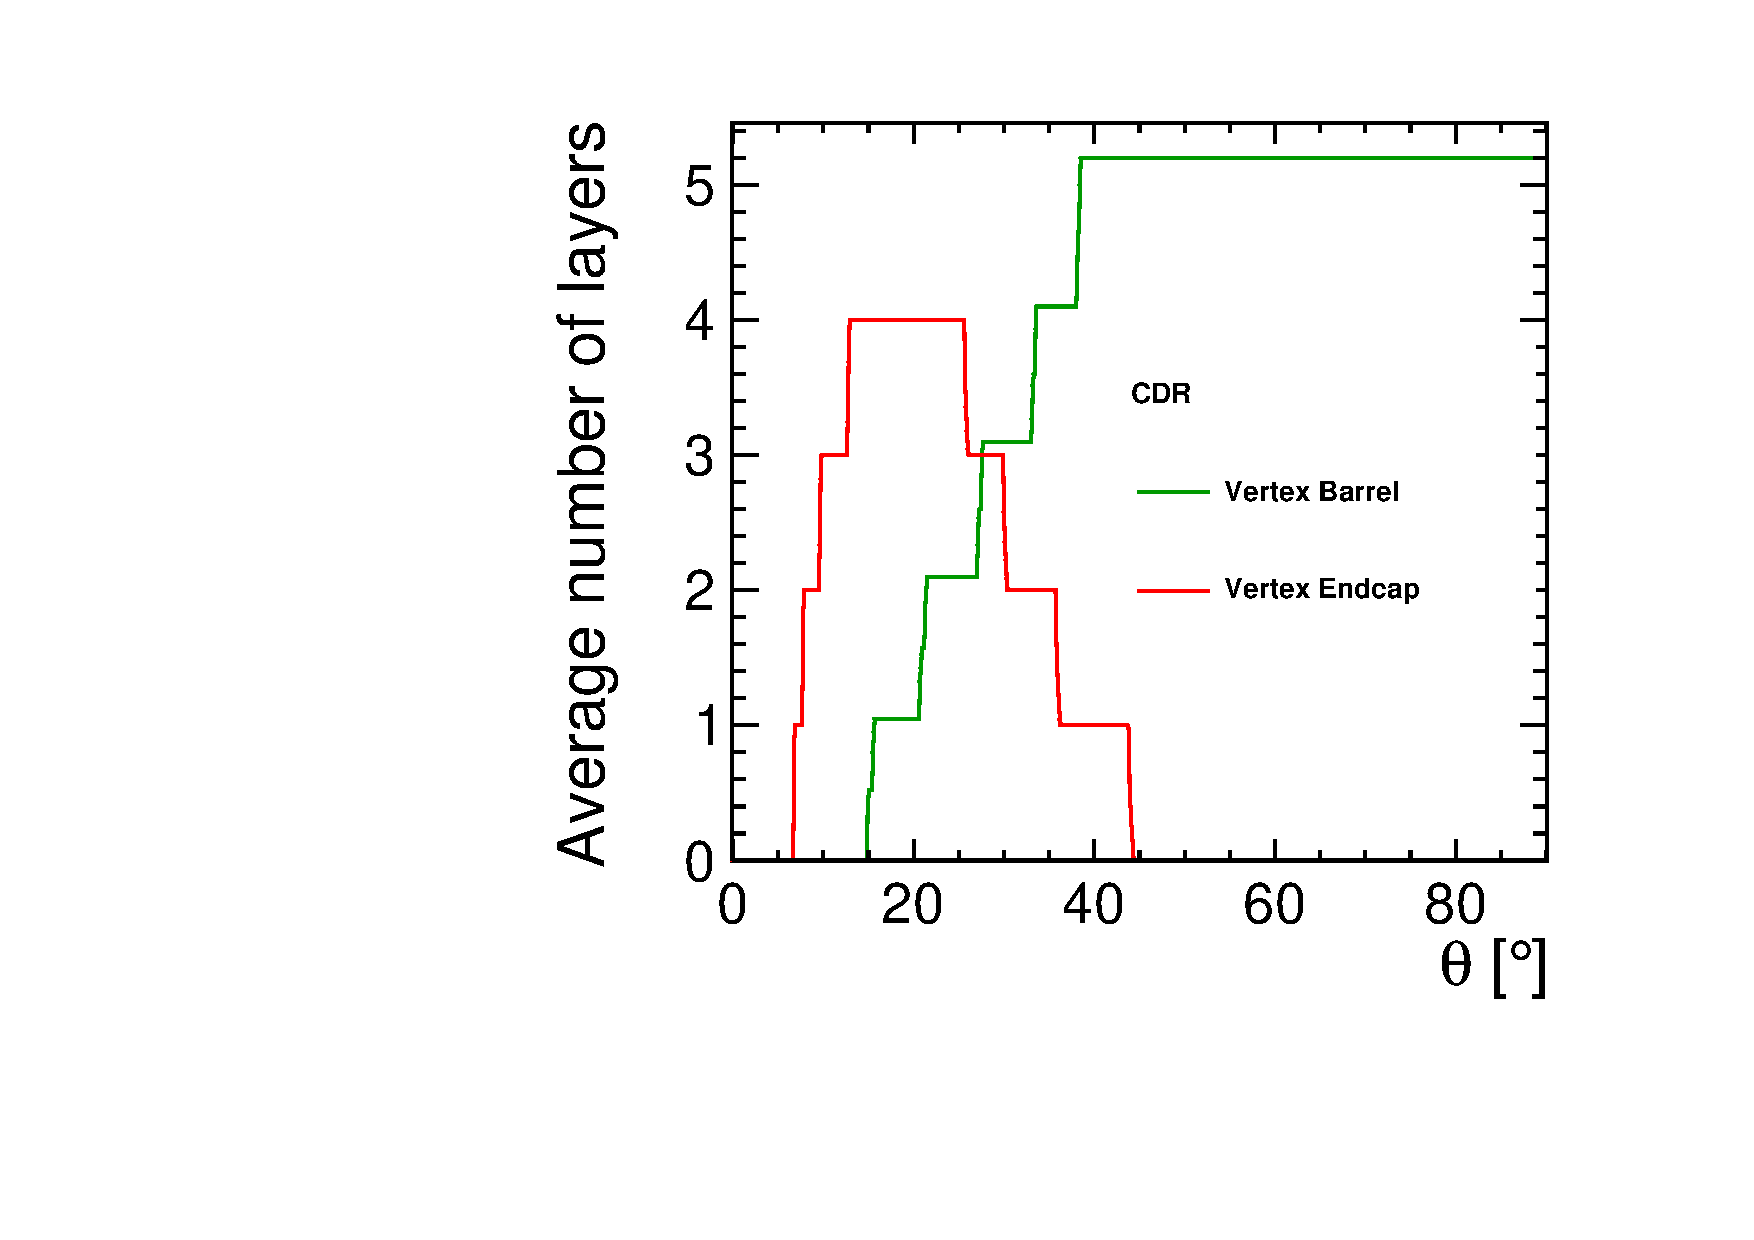
\includegraphics[scale=0.4]{Figures/Geometries/nb_layer_cdr.pdf}
  \caption{The coverage of the vertex detector with respect to the polar angle $\theta$ for the CDR geometry. The number of layers is averaged over the azimuthal angle $\phi$.}
  \label{fig:default_nb_barrel_endcap}
\end{figure}

%----------------------------------------------------------------------
\subsection{The \emph{spirals} geometry}\label{sec:CLIC_SiD_spirals}

Several engineering studies are in progress to limit the material, e.g. the cables, the mechanical support and also the cooling. Cooling solutions with pipes and liquids increase significantly the material budget. The aim is therefore to use airflow cooling for the CLIC vertex detector. \\
However, the CDR geometry was not designed for the airflow cooling. The vertex endcaps, which are made of disks, do not allow the air to flow through the vertex detector. \\
One solution is to use a spiral arrangement for the modules in the endcap regions~\cite{CoolingSimulations}. Figure~\ref{fig:spirals_cooling_simulations} illustrates the airflow cooling concept for the vertex detector. The air can flow through the endcap on one side, continue along the barrel sensors and flow out through the other endcap.

%% \begin{figure}[H]
%%   \centering
%%   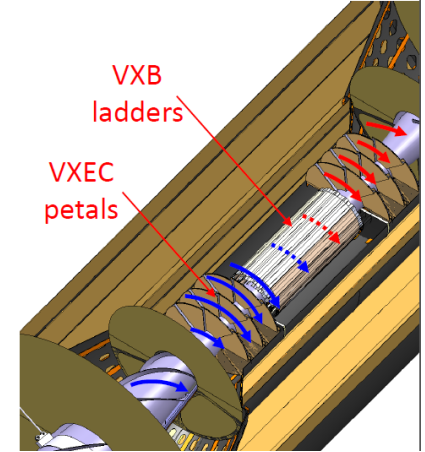
\includegraphics[scale=0.3]{Figures/Geometries/airflow.png}
%%   \caption{Engineering model for the vertex detector with spiral endcap disks: the air flows into the endcap on one side and out from the other endcap passing the barrel region.}\label{fig:spirals_cooling_simulations}
%% \end{figure}

\begin{figure}[H]
  \centering
  \includegraphics[page=8, trim = 20mm 85mm 20mm 155mm, clip, width=\textwidth]{Figures/LCD-Note-cooling.pdf}
  \caption{Engineering sketch showing the airflow cooling strategy within the vertex detector. From~\cite{CoolingSimulations}.}\label{fig:spirals_cooling_simulations}
\end{figure}

The parameters for the spiral arrangement of the sensors in the vertex endcaps are given in Table~\ref{tab:params_spiral_endcap}. For this geometry the number of trapezoidal modules \textit{N} in a layer is reduced to 8 compared to 16 for the CDR geometry. In Table~\ref{tab:params_spiral_endcap}, \textit{z} gives the distance of the first module of each layer to the interaction point in the vertex endcaps and the modules are interspaced by a distance of $\Delta z$=3.6~mm. The first module in each layer covers the azimuthal angle from $\phi=157.5^{\circ}$ to $\phi=202.5^{\circ}$.\\
Figure~\ref{fig:singleSpiralGeom} shows the \begin{it}spirals\end{it} geometry as implemented in the simulations. The barrel geometry is identical to the one of the CDR geometry. 

\begin{table}[H]
  \caption{Parameters for the trapezoidal modules in the endcap regions
    of the {\it spirals} geometry, where \textit{N} represents the
    number of modules in a layer, $r_{in}$ and $r_{out}$ the inner and
    the outer radius at the outer edge of the trapezoidal modules,
    $w_{in}$ and $w_{out}$ the inner and the outer widths, \textit{z}
    the position of the first module of the layer. The other modules are placed at a distance of $\Delta$\textit{z}=3.6~mm from the previous module in the \textit{z} direction. In the \textsc{Geant4} simulations, each module is made of \SI{50}{\micro\meter} of silicon followed by \SI{130}{\micro\meter} of carbon fiber.}
  \begin{center}
    \begin{tabular}{ c c c c c c c }
      \hline
      Layer & N & r$_{in}$[mm] & r$_{out}$[mm] & w$_{in}$[mm] & w$_{out}$[mm] & z[mm] \\ \hline \hline
      1 & 8 & 27.0 & 115.0 & 22.7 & 96.6 & 120.0 \\ \hline
      2 & 8 & 27.0 & 115.0 & 22.7 & 96.6 & 150.0 \\ \hline
      3 & 8 & 27.0 & 115.0 & 22.7 & 96.6 & 180.0 \\ \hline
      4 & 8 & 28.1 & 115.0 & 23.6 & 96.6 & 210.0\\ \hline
    \end{tabular}
  \end{center}
  \label{tab:params_spiral_endcap}
\end{table}

\begin{figure}[H]
  \centering
  \begin{tikzpicture}
    \node[anchor=south west,inner sep=0] (image) at (0,0){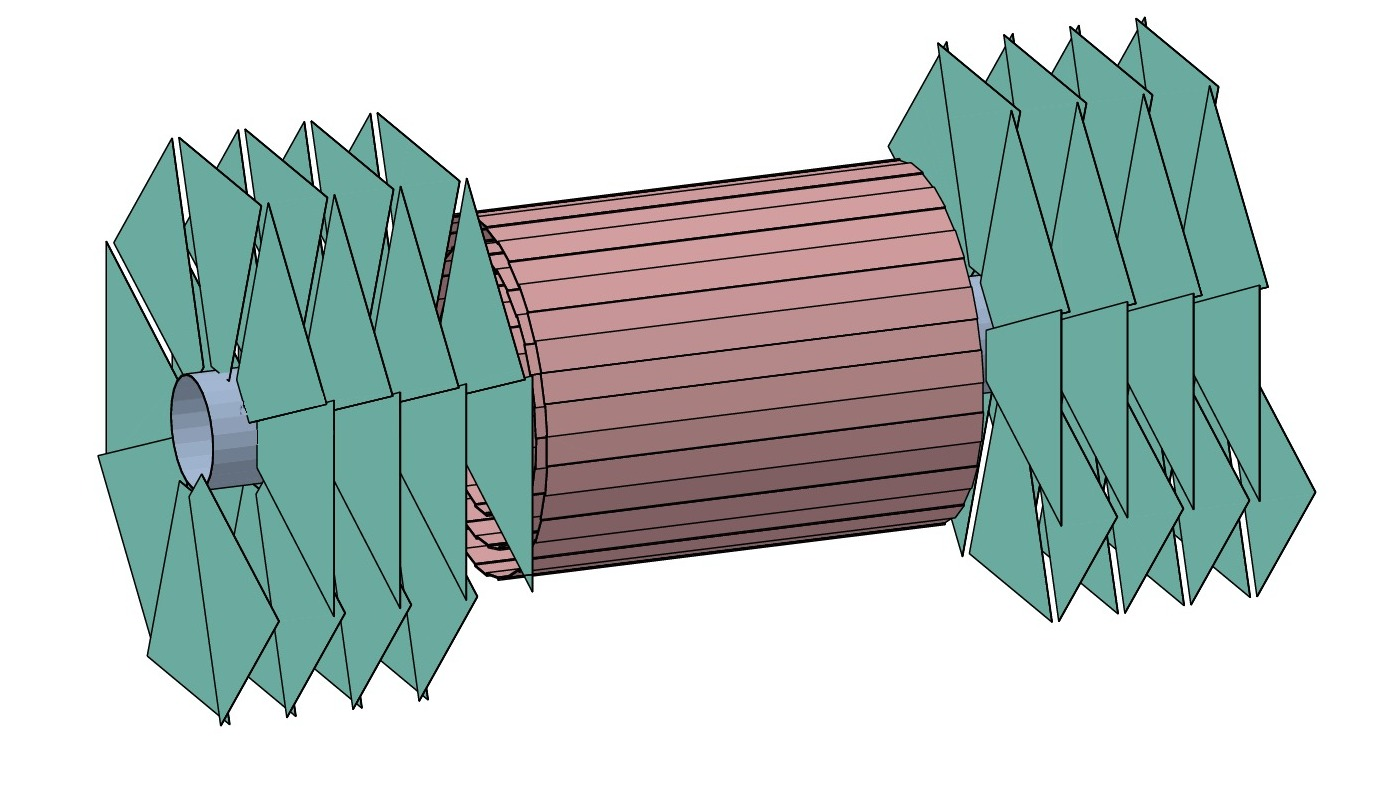
\includegraphics[width=15cm]{Figures/Geometries/single_spiral.jpg}};
    \draw[->,line width=.4pt, color=ForestGreen](15, 5) -- (15, 7);
    \node[right, color=ForestGreen] at (15, 7) {$y$};
    \draw[->,line width=.4pt, color=ForestGreen](15, 5) -- (16.6, 5.2);
    \node[right, color=ForestGreen] at (16.6, 5.2) {$z$};
    \draw[->,line width=.4pt, color=ForestGreen](15, 5) -- (13.7, 5.6);
    \node[right, color=ForestGreen] at (13.7, 5.6) {$x$};
  \end{tikzpicture}
  \caption{Schematic view of the vertex detector for the {\it spirals} geometry. The barrel is shown in red and is the same as the CDR barrel. The vertex endcaps modules are shown in green.}
  \label{fig:singleSpiralGeom}
\end{figure}

To minimise the effect of multiple scattering, a low material budget is required for the vertex detector. Figure~\ref{fig:materialBudgSpiralEndcap} compares the material budget for the CDR and the \begin{it}spirals\end{it} geometries. For the computation of the material budget we integrate from the interaction point to the outside of the highlighted areas in Figure~\ref{fig:endcap_placement}, including the beam pipe and cabling. For each polar angle $\theta$, the material budget is averaged over the azimuthal angle $\phi$. As shown in Figure~\ref{fig:materialBudgSpiralEndcap}, the amount of material does not differ much for the \begin{it}spirals\end{it} geometry compared to the CDR layout (the large peak at low polar angles corresponds to the beam pipe).  \\
The number of silicon layers as a function of the polar angles $\theta$ averaged over $\phi$ is given in Figure~\ref{fig:spiral_nb_barrel_endcap} and is very similar for the CDR and the \begin{it}spirals\end{it} geometries. The main difference compared to the disks (see Figure~\ref{fig:default_nb_barrel_endcap}) is that the number of layers varies with the $\phi$ angle.


\begin{figure}[H]
  \begin{subfigure}[b]{0.5\textwidth}
    \centering
    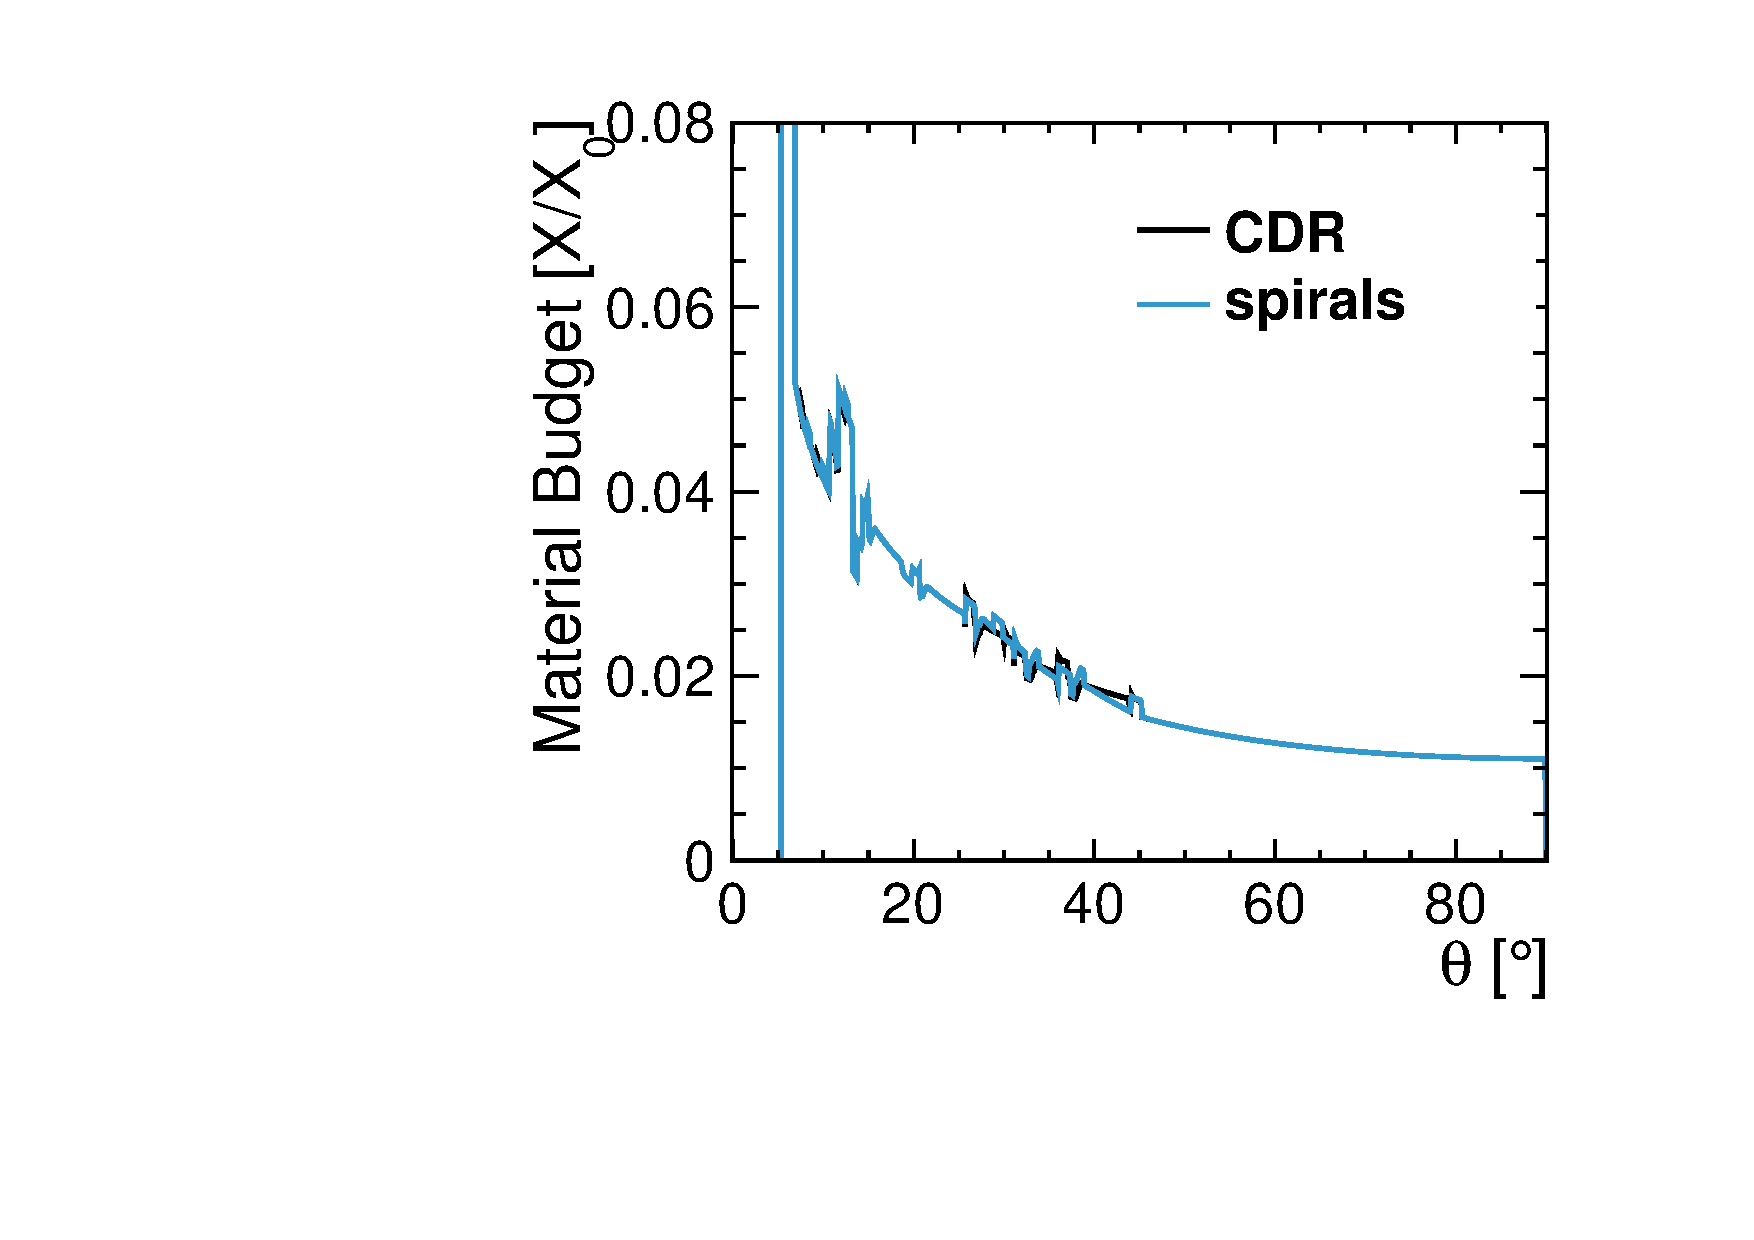
\includegraphics[scale=0.4]{Figures/Geometries/material_budget_spirals.pdf}
    \caption{}\label{fig:materialBudgSpiralEndcap}
  \end{subfigure}~
  \begin{subfigure}[b]{0.5\textwidth}
    \centering
    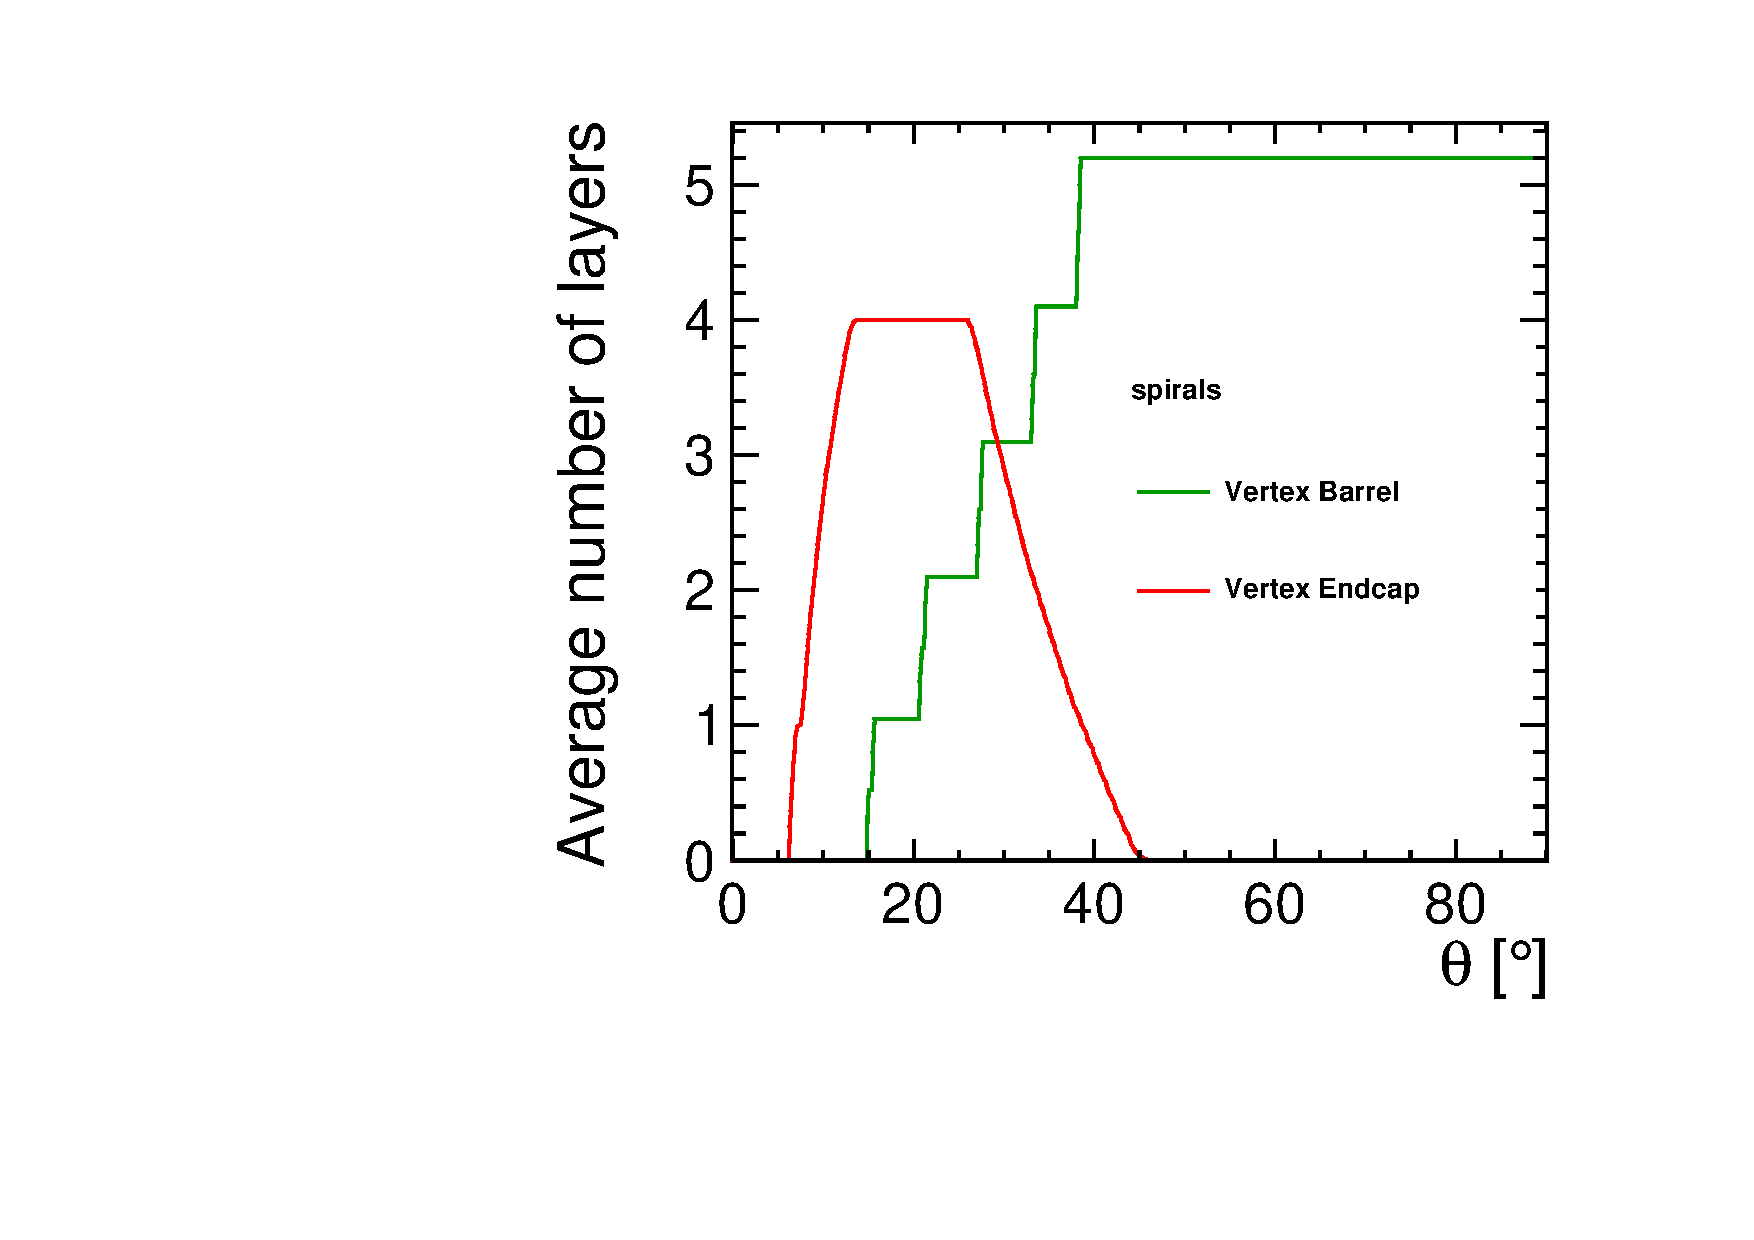
\includegraphics[scale=0.4]{Figures/Geometries/nb_layer_spirals.pdf}
    \caption{}\label{fig:spiral_nb_barrel_endcap}
  \end{subfigure}
  \caption{The material budget for the CDR and the {\it spirals} vertex detectors is shown in (a). The coverage of the vertex detector for the {\it spirals} geometry with respect to the polar angle $\theta$ is shown in (b). The material budget and the number of layers for each polar angle $\theta$ are averaged over the azimuthal angle $\phi$.}
\end{figure}


%----------------------------------------------------------------------
\subsection{The \emph{double\_spirals} geometry}\label{sec:CLIC_SiD_double_spirals}

In the vertex detector, we would like to have as many measurement points as possible and, at the same time, minimise the amount of material. The \begin{it}double\_spirals\end{it} geometry uses two silicon sensors on either side of a single mechanical support in the barrel and the endcap regions. As airflow is foreseen for the heat removal of the detector, a spiral arrangement of the modules is used in the endcap regions as in Section~\ref{sec:CLIC_SiD_spirals}. \\
In the barrel region, the five layers of single-sided modules are replaced by three layers of double-sided modules. Similarly, in the vertex endcaps, instead of four single layers, there are three double layers in a spiral arrangement.\\
Both sides of each module contain silicon sensors with a thickness of \SI{50}{\micro\meter} (cf. Figure~\ref{fig:DL_vertex_barrel_b}). The overall thickness of the carbon fiber used to emulate the mechanical support, cabling and the electronics is \SI{130}{\micro\meter} (each silicon sensor is followed by \SI{65}{\micro\meter} carbon fiber support) and the rest of the module is filled with air. The overall thickness of a double-layer module is \SI{2}{\milli\meter} and is based on the CLIC\_ILD\_CDR layout~\cite{Muennich:1443543} with a material budget of $0.18\%X_{0}$. A schematic view of the double-layered sensor as implemented in the simulations is shown in Figure~\ref{fig:DL_vertex_barrel}. The thickness of the carbon per module layer is the same as the one used for the CDR geometry as we assume that the same amount of support structure and cables is used for the single and the double-layered sensors. The parameters of the \begin{it}double\_spirals\end{it} geometry are given in Tables \ref{tab:params_DL} and \ref{tab:params_double_endcap}.
Figure~\ref{fig:doubleSpiralGeom} illustrates the vertex detector
implemented with double-layered sensors.
\begin{table}[H]
  \caption{Parameters of the vertex barrel layers for the {\it
      double\_spirals} geometry, where \textit{N} represents the
    number of modules in a layer, \textit{r} is the mean radius of the
    layer, \textit{z} the half-length of the module and \textit{w} is
    the width of the module. Each module is made of two layers of
    silicon sensors with a thickness of \SI{50}{\micro\meter} plus \SI{65}{\micro\meter} of carbon fiber.}
  \label{tab:params_DL}
  \begin{center}
    \begin{tabular}{ c c c c c }
      \hline
      Layer & N & r[mm] & z[mm] & w[mm]\\ \hline \hline
      1 & 18 & 27.0 & 98.5 & 9.8 \\ \hline
      2 & 24 & 51.0 & 98.5 & 13.8 \\ \hline
      3 & 36 & 77.0 & 98.5 & 13.8 \\ \hline
    \end{tabular}
  \end{center}  
\end{table}

\begin{table}[H]
  \caption{Parameters for the trapezoidal modules of the {\it
      double\_spirals} geometry in the endcap regions, where
    \textit{N} represents the number of modules in a layer, $r_{in}$
    and $r_{out}$ the inner and the outer radius for the disks at the
    outer edge of the trapezoidal modules, \textit{z} the position of
    the first module of the layer. The other modules are placed at a
    distance of $\Delta z$=5~mm from the previous module in the
    \textit{z} direction. For the trapezoidal modules, $w_{in}$ and
    $w_{out}$ represent the inner and the outer widths. Each module is
    made of two layers of silicon sensors with a thickness of
    \SI{50}{\micro\meter} plus \SI{65}{\micro\meter} of carbon fiber.}
  \begin{center}
    \begin{tabular}{ c c c c c c c }
      \hline
      Layer & N & r$_{in}$[mm] & r$_{out}$[mm] & w$_{in}$[mm] & w$_{out}$[mm] & z[mm] \\ \hline \hline
      1 & 8 & 27.0 & 115.0 & 22.7 & 96.6 & 120.0 \\ \hline
      2 & 8 & 27.0 & 115.0 & 22.7 & 96.6 & 160.0 \\ \hline
      3 & 8 & 27.0 & 115.0 & 22.7 & 96.6 & 200.0 \\ \hline
    \end{tabular}
  \end{center}
  \label{tab:params_double_endcap}
\end{table}

\vspace{-0.2cm}

\begin{figure}[H]
  \begin{subfigure}[]{0.5\textwidth}
    \centering
    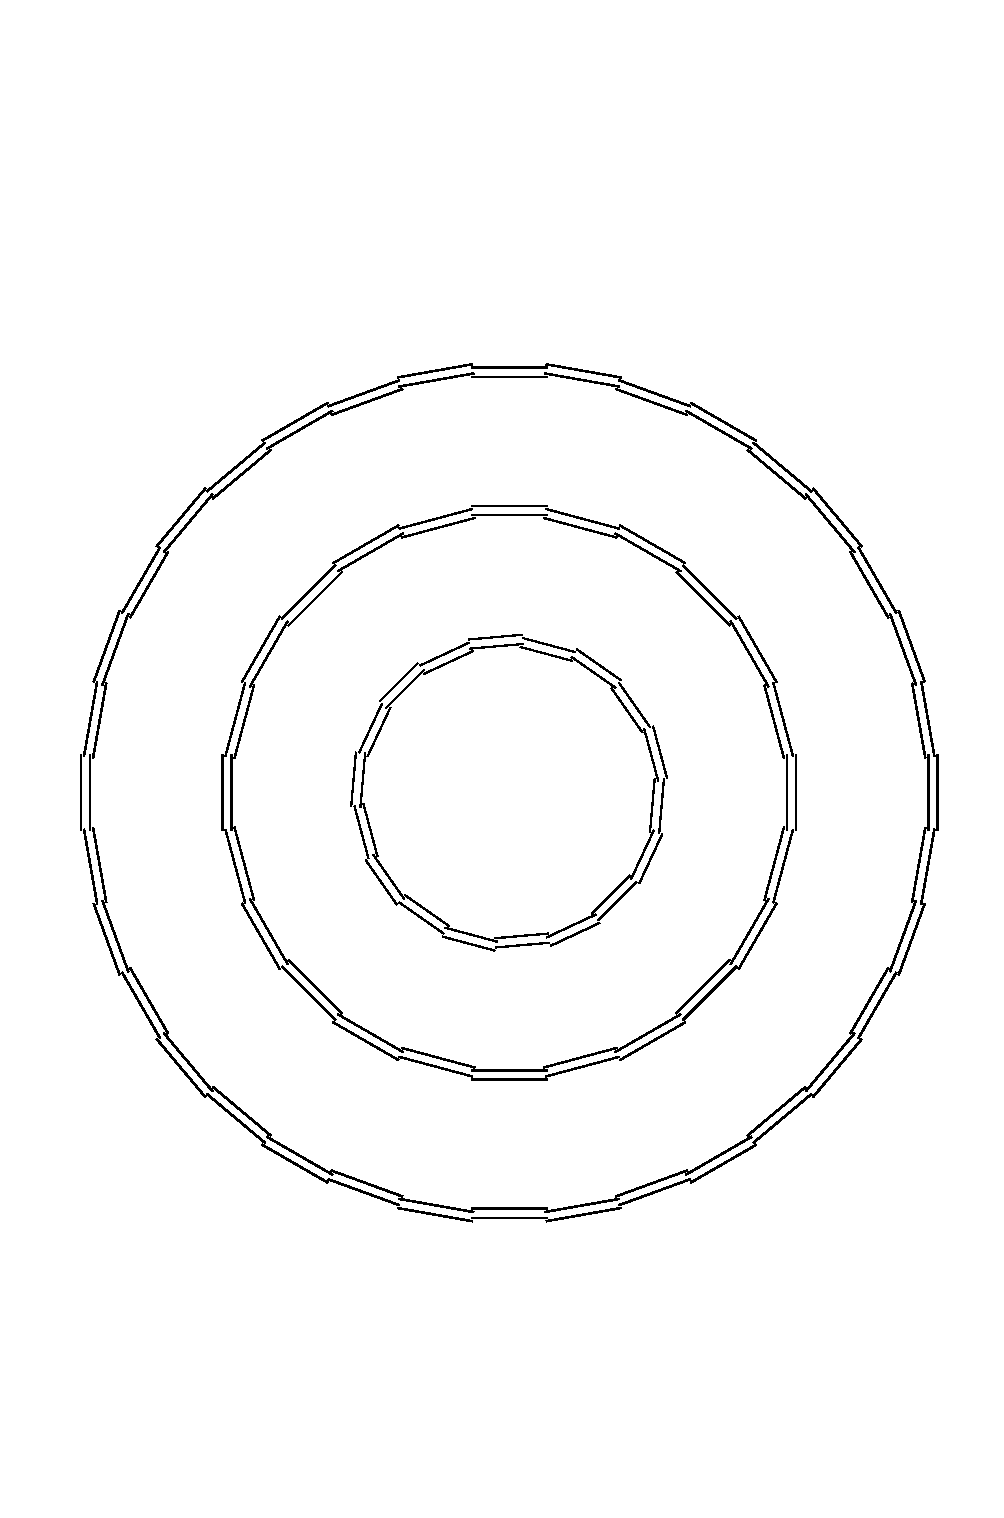
\includegraphics[trim = 0mm 30mm 0mm 30mm, clip, width=7cm]{Figures/Geometries/double_barrel_module.pdf}\caption{}\label{fig:DL_vertex_barrel_a}
  \end{subfigure}~
  \begin{subfigure}[c]{0.5\textwidth}
    \vspace{6.5cm}
    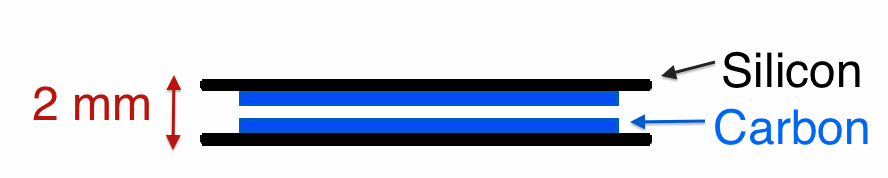
\includegraphics[width=\textwidth]{Figures/Geometries/double_layer_module.png}\caption{}\label{fig:DL_vertex_barrel_b}
    % \vspace{-2cm}
    % \begin{tikzpicture}
    %   \node[anchor=south west,inner sep=0] at (0,0){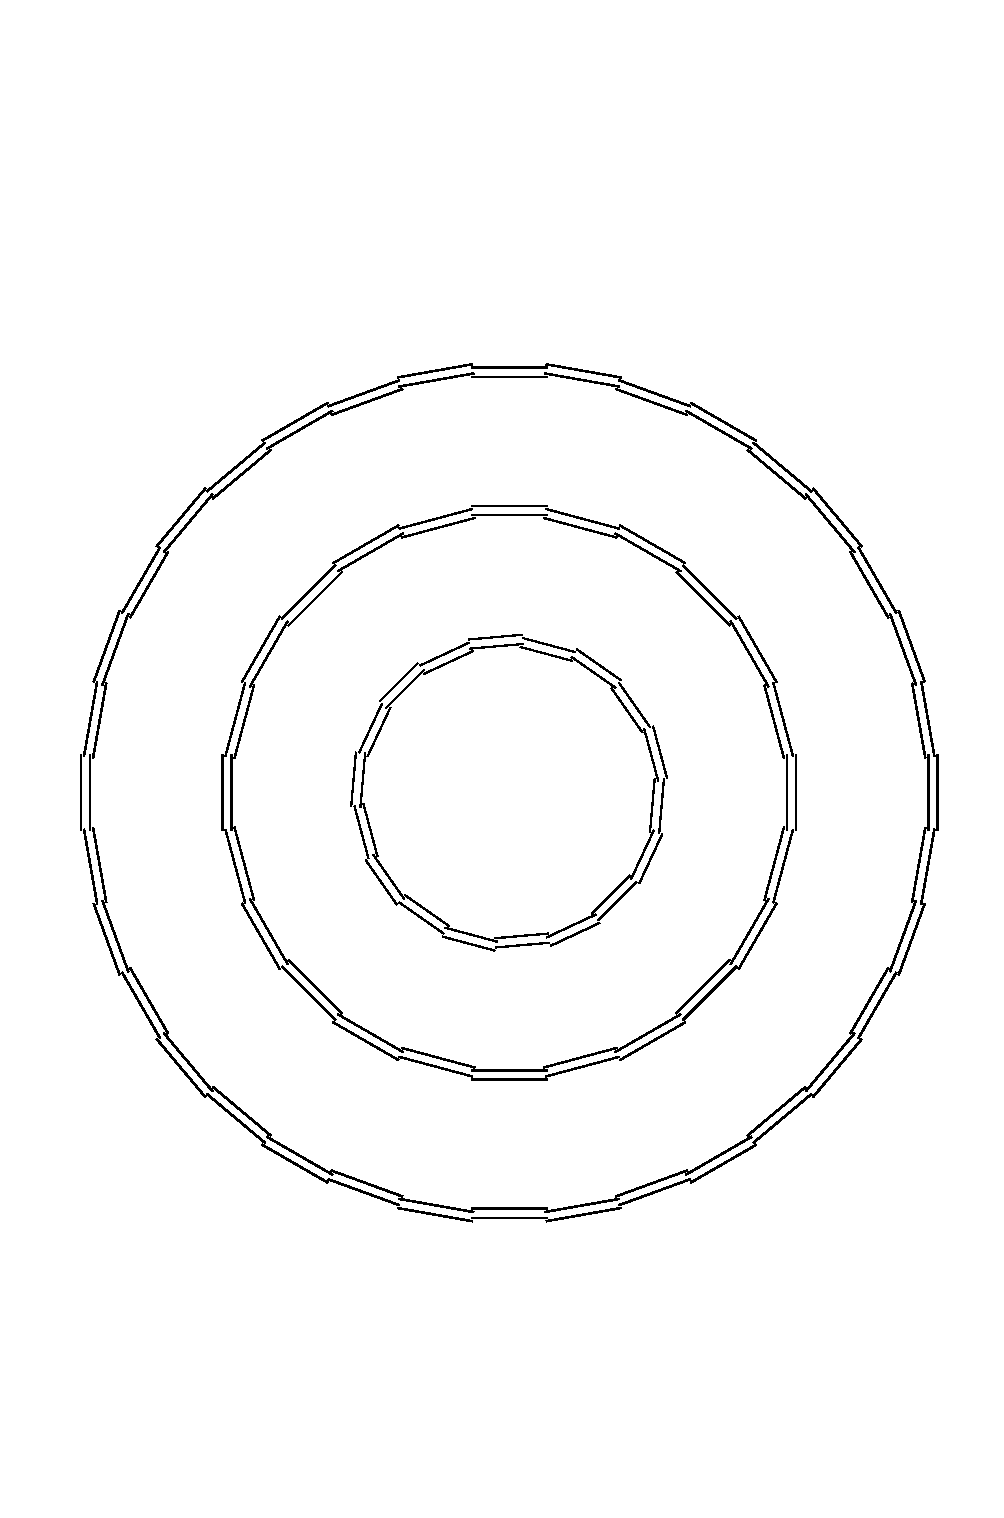
\includegraphics[trim = 75mm 50mm 73mm 200mm, clip, width=7cm]{Figures/Geometries/double_barrel_module.pdf}};
    %   \draw[<->,line width=.4pt, red, thick](3.5,0.2) to node[midway, xshift=0.7cm, red]{2 mm} (3.5,0.86);
    % \end{tikzpicture}
    % \label{fig:DLzoom_vertex_barrel}
  \end{subfigure}
    \caption{The schematic view of the vertex barrel of the {\it double\_spirals} geometry is shown in (a). In the \textsc{Geant4} simulations, each module is implemented as two silicon sensors on top of each other and the overall thickness of the module is \SI{2}{\milli\meter} as illustrated in (b). }\label{fig:DL_vertex_barrel}
\end{figure}

\begin{figure}[H]
  \centering
  \begin{tikzpicture}
    \node[anchor=south west,inner sep=0] (image) at (0,0){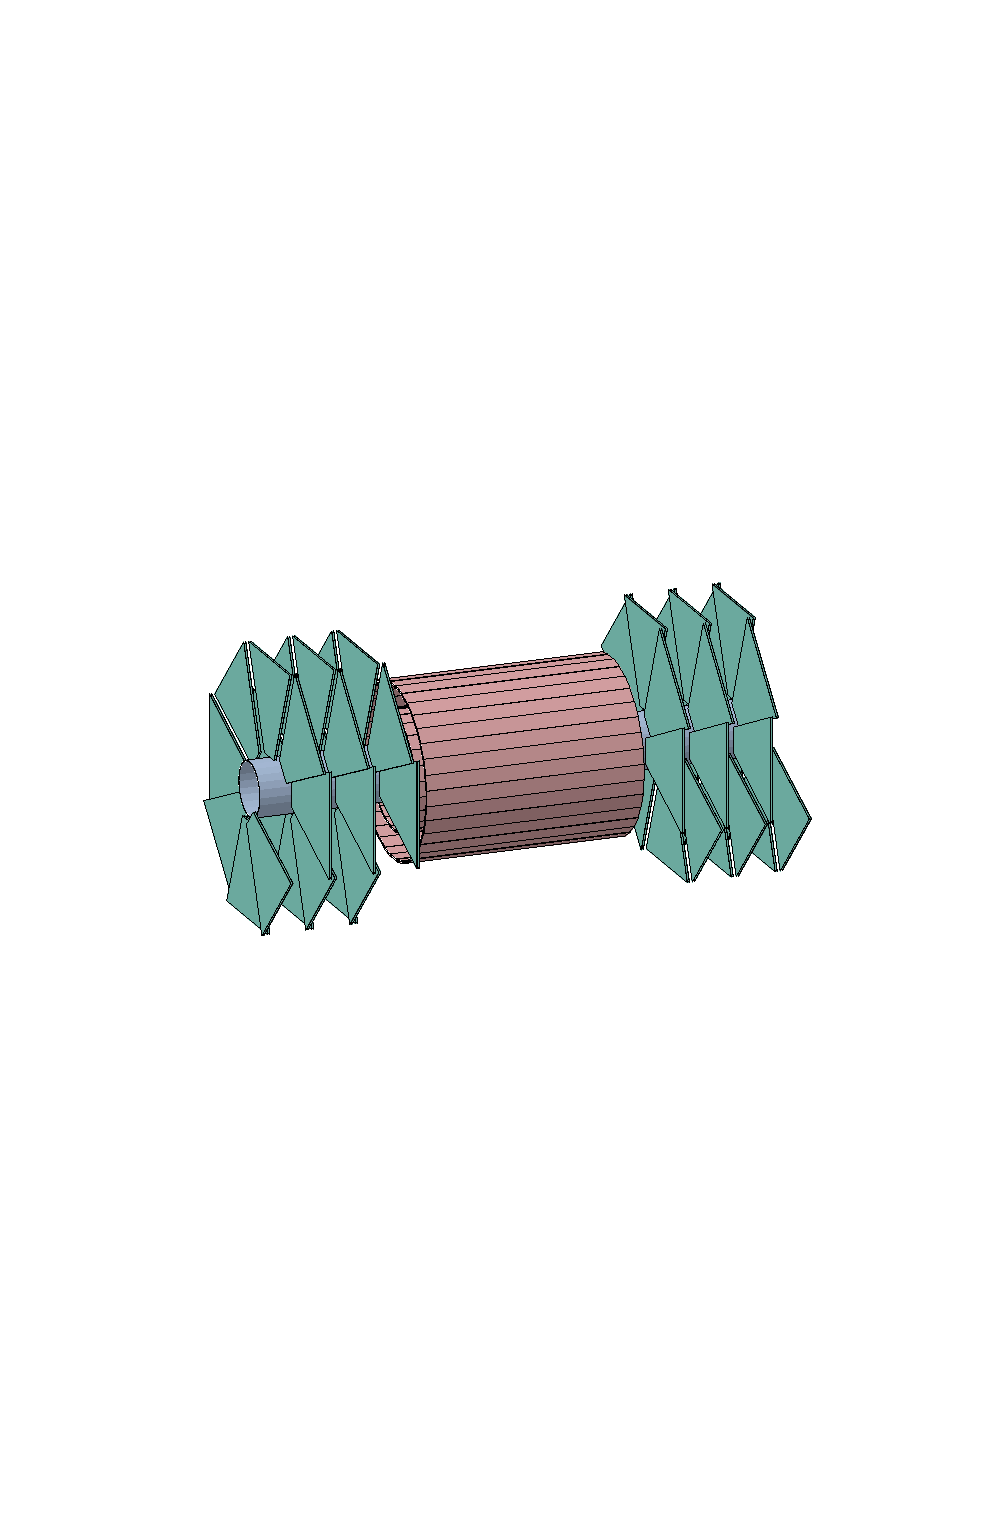
\includegraphics[trim = 20mm 98mm 20mm 90mm, clip, width=15cm]{Figures/Geometries/double_spiral.pdf}};
    \draw[->,line width=.4pt, color=ForestGreen](15, 5) -- (15, 7);
    \node[right, color=ForestGreen] at (15, 7) {$y$};
    \draw[->,line width=.4pt, color=ForestGreen](15, 5) -- (16.6, 5.2);
    \node[right, color=ForestGreen] at (16.6, 5.2) {$z$};
    \draw[->,line width=.4pt, color=ForestGreen](15, 5) -- (13.7, 5.6);
    \node[left, color=ForestGreen] at (13.7, 5.6) {$x$};
  \end{tikzpicture}
  \caption{Schematic view of the vertex detector for the {\it double\_spirals} geometry. The barrel region is shown in red and the vertex endcaps in green.}
  \label{fig:doubleSpiralGeom}
\end{figure}

The material budget for the {\it double\_spirals} geometry is shown in Figure~\ref{fig:materialBudgSpiralEndcap_double} and is very similar to the CDR geometry. The amount of silicon layers has increased but overall less carbon is needed for the mechanical support. \\
Figure~\ref{fig:double_nb_barrel_endcap} shows the coverage of the {\it double\_spirals} geometry. The average number of layers in the vertex endcaps is higher than for the CDR and the \begin{it}spirals\end{it} geometries with similar material budget (see Figures \ref{fig:default_nb_barrel_endcap} and \ref{fig:spiral_nb_barrel_endcap}). 

\begin{figure}[H]
  \begin{subfigure}[b]{0.5\textwidth}
    \centering
    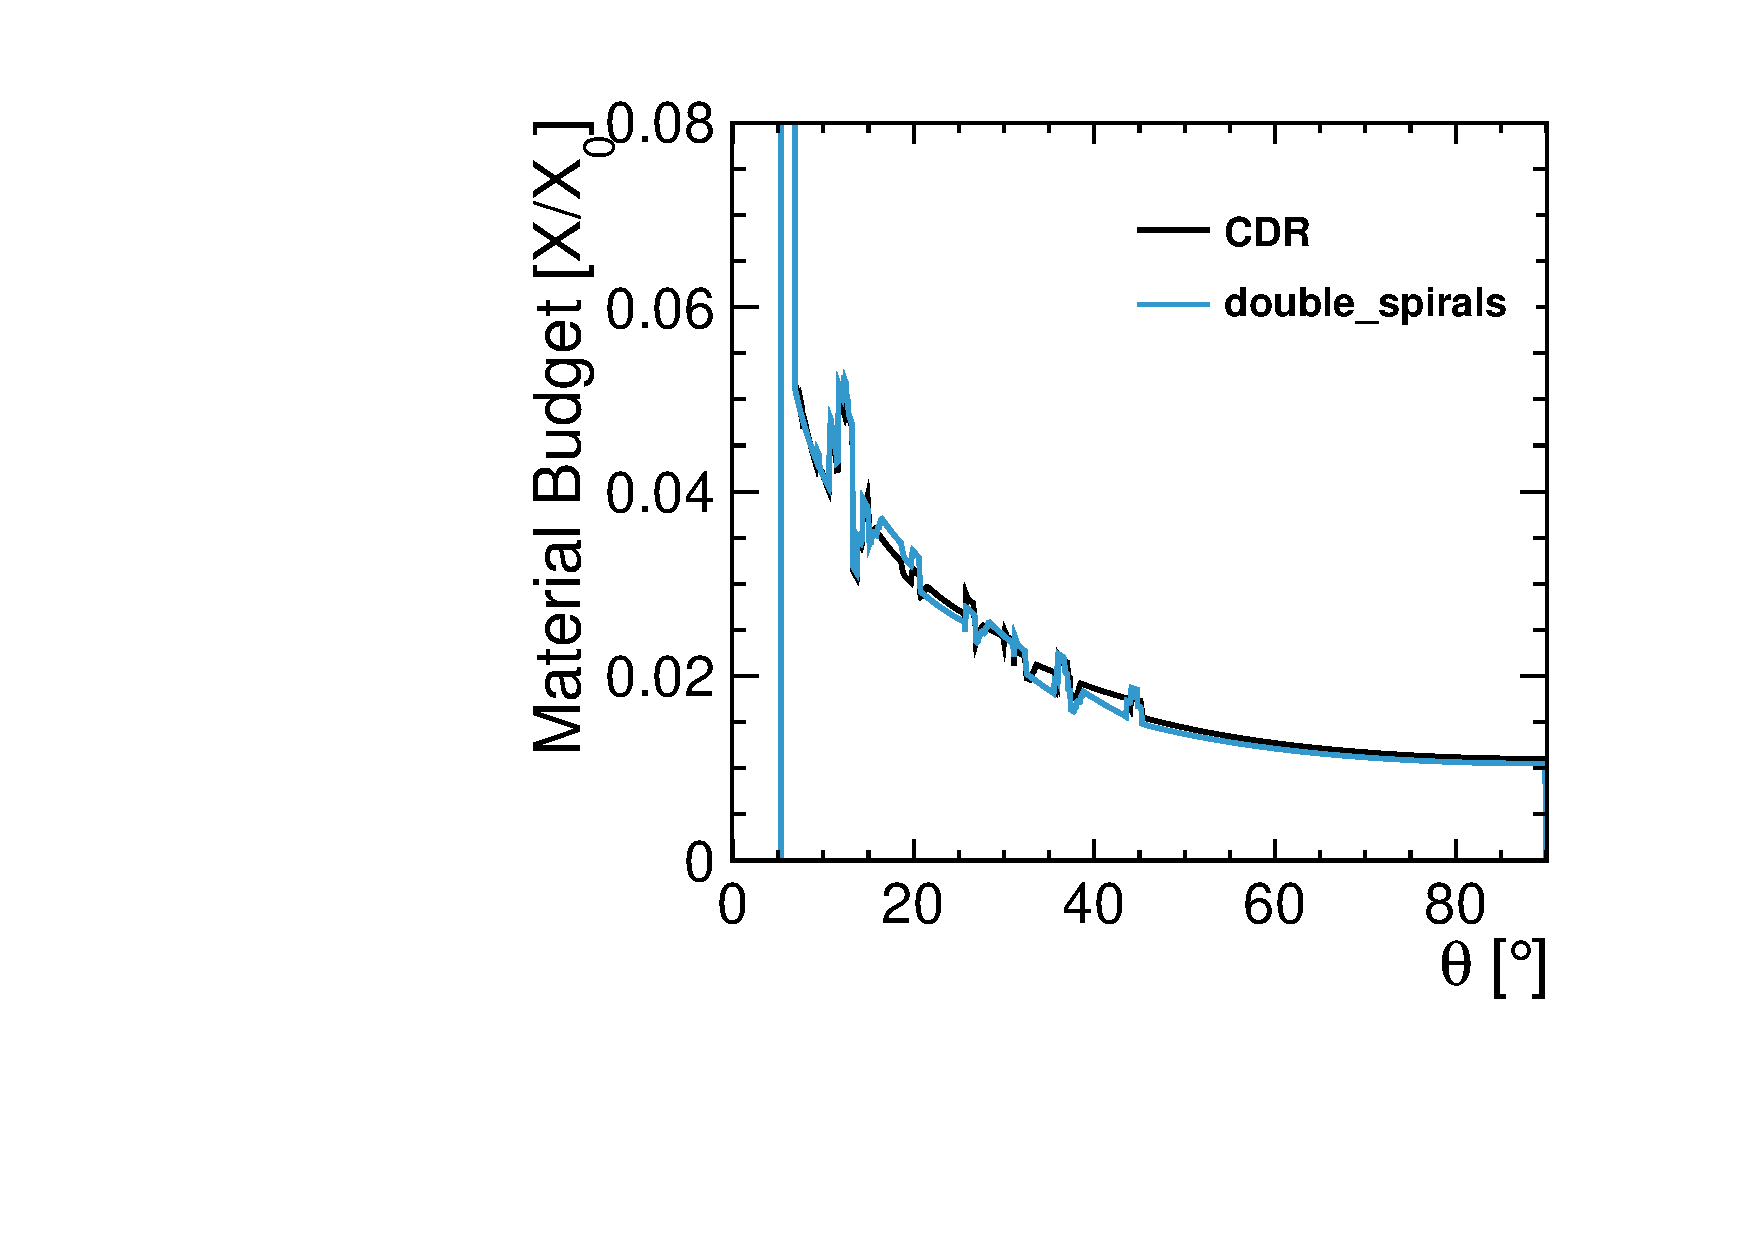
\includegraphics[scale=0.4]{Figures/Geometries/material_budget_double_spirals.pdf}
    \caption{}\label{fig:materialBudgSpiralEndcap_double}
\end{subfigure} \quad
  \begin{subfigure}[b]{0.5\textwidth}
    \centering
    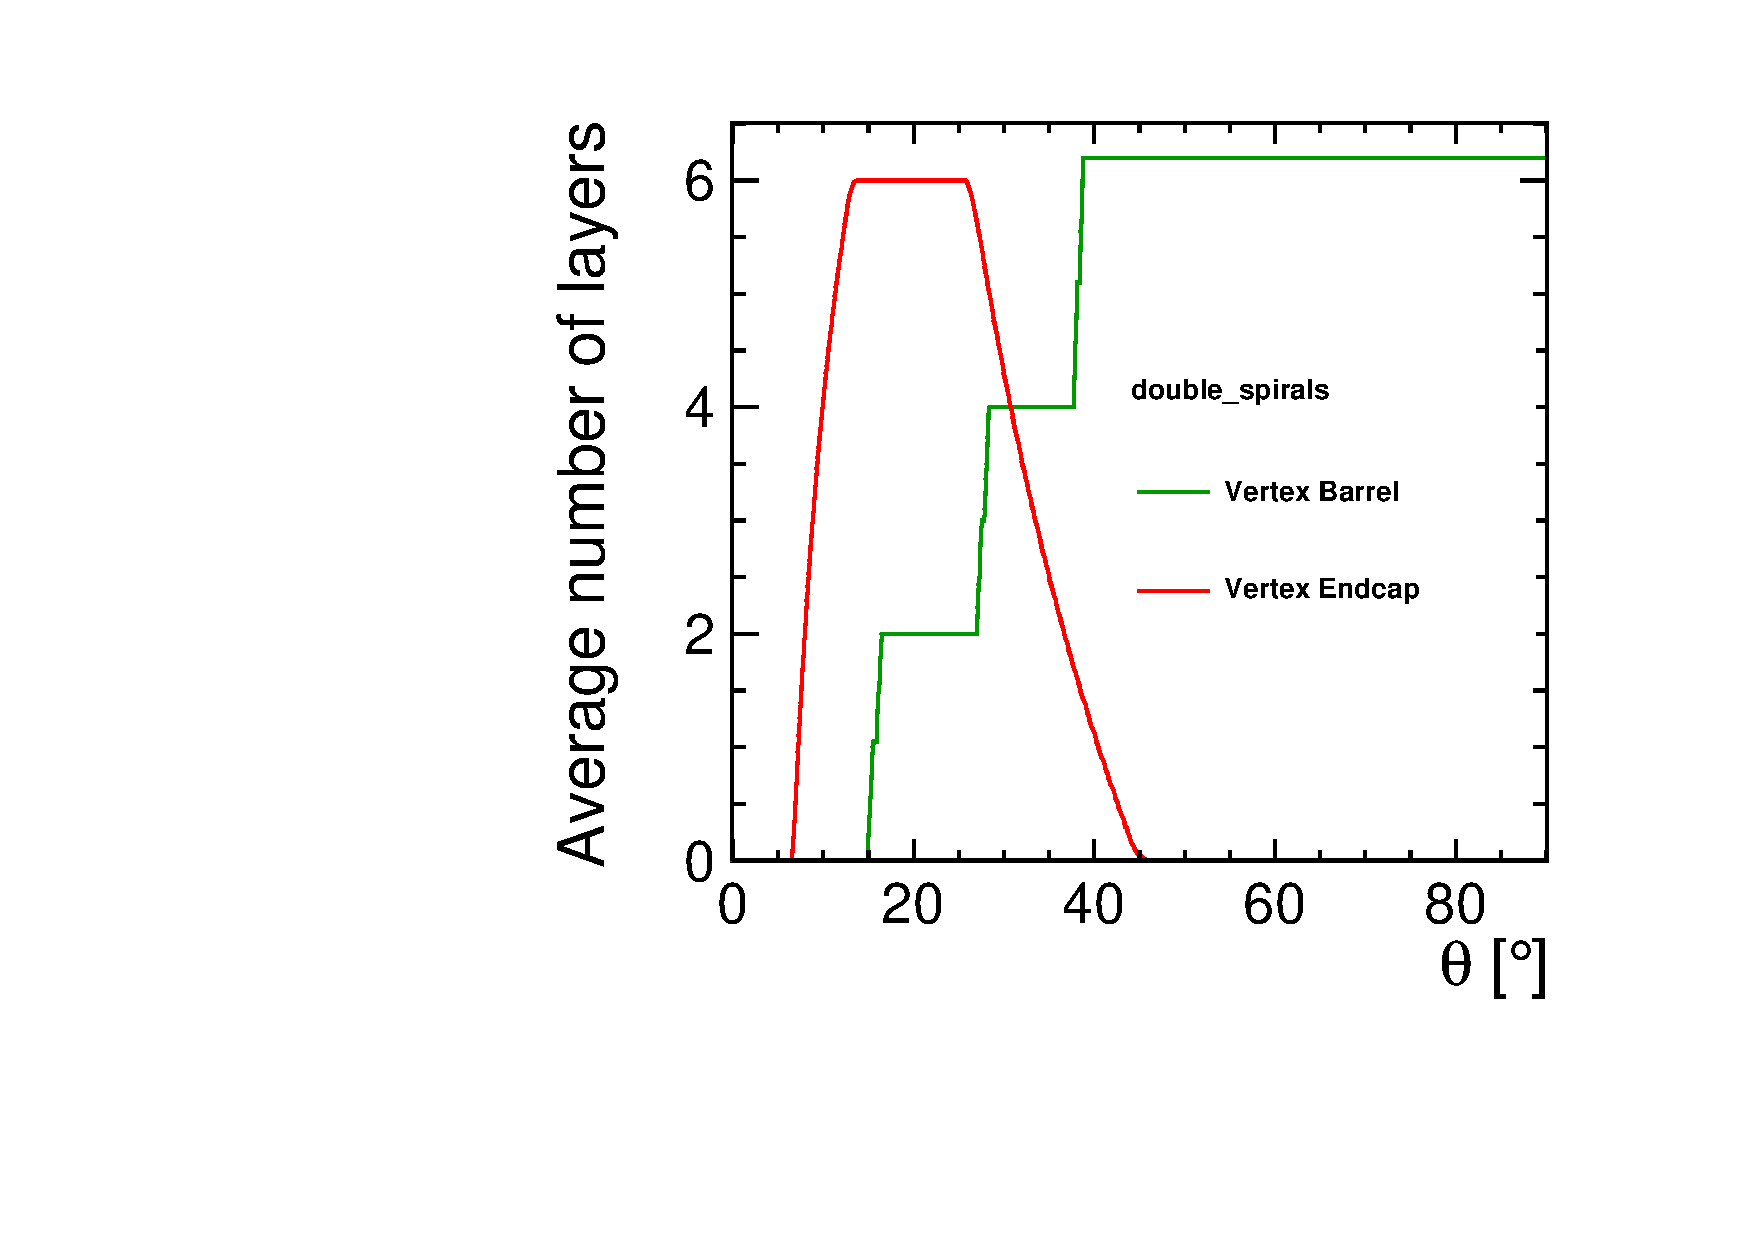
\includegraphics[scale=0.4]{Figures/Geometries/nb_layer_double.pdf}
    \caption{}\label{fig:double_nb_barrel_endcap}
  \end{subfigure}
  \caption{The material budget for the CDR and the {\it double\_spirals} vertex detectors is shown in (a). The coverage of the vertex detector for the {\it double\_spirals} geometry with respect to the polar angle $\theta$ is shown in (b). The material budget and the number of layers for each polar angle $\theta$ are averaged over the azimuthal angle $\phi$.}
\end{figure}

\newpage
As a cross-check, we have also calculated the material budget for both geometries at a polar angle of $\theta = 90^{\circ}$ using the thicknesses of all the material used. The calculated and the simulated values are compared in Table~\ref{tab:material_budg_DL_table}. We can observe that both values are quite similar, but the simulation gives higher values. This can be explained by the fact that for the simulation, the material budget is integrated over the $\phi$ angle and for some azimuthal angles the modules overlap. The calculation, on the other hand, does not consider these overlaps. 

\begin{table}[H]
  \caption{Calculated and simulated values of the material budget for the CDR and the \textit{double\_spirals} vertex barrel at $\theta = 90^{\circ}$ in units of $X_{0}$.}
  \begin{center}
    \begin{tabular}{ c  c  c } \hline
      & CDR & \textit{double\_spirals} \\  \hline \hline
      Calculation & $1.07\%$ & $1.00\%$ \\ \hline
      Simulation & $1.10\%$ & $1.05\%$ \\ \hline
    \end{tabular}
  \end{center}
  \label{tab:material_budg_DL_table}
\end{table}


Figure~\ref{fig:vertex_nb_layer} summarizes the coverage of the whole vertex detector (the vertex barrel and endcaps) for the above-mentioned geometries with respect to the polar angle $\theta$ (averaged over $\phi$). Overall, the \begin{it}double\_spirals\end{it} geometry has more sensitive layers in the barrel and the endcaps with similar material budget as the CDR and the \begin{it}spirals\end{it} geometries. 


\begin{figure}[H]
  \centering
  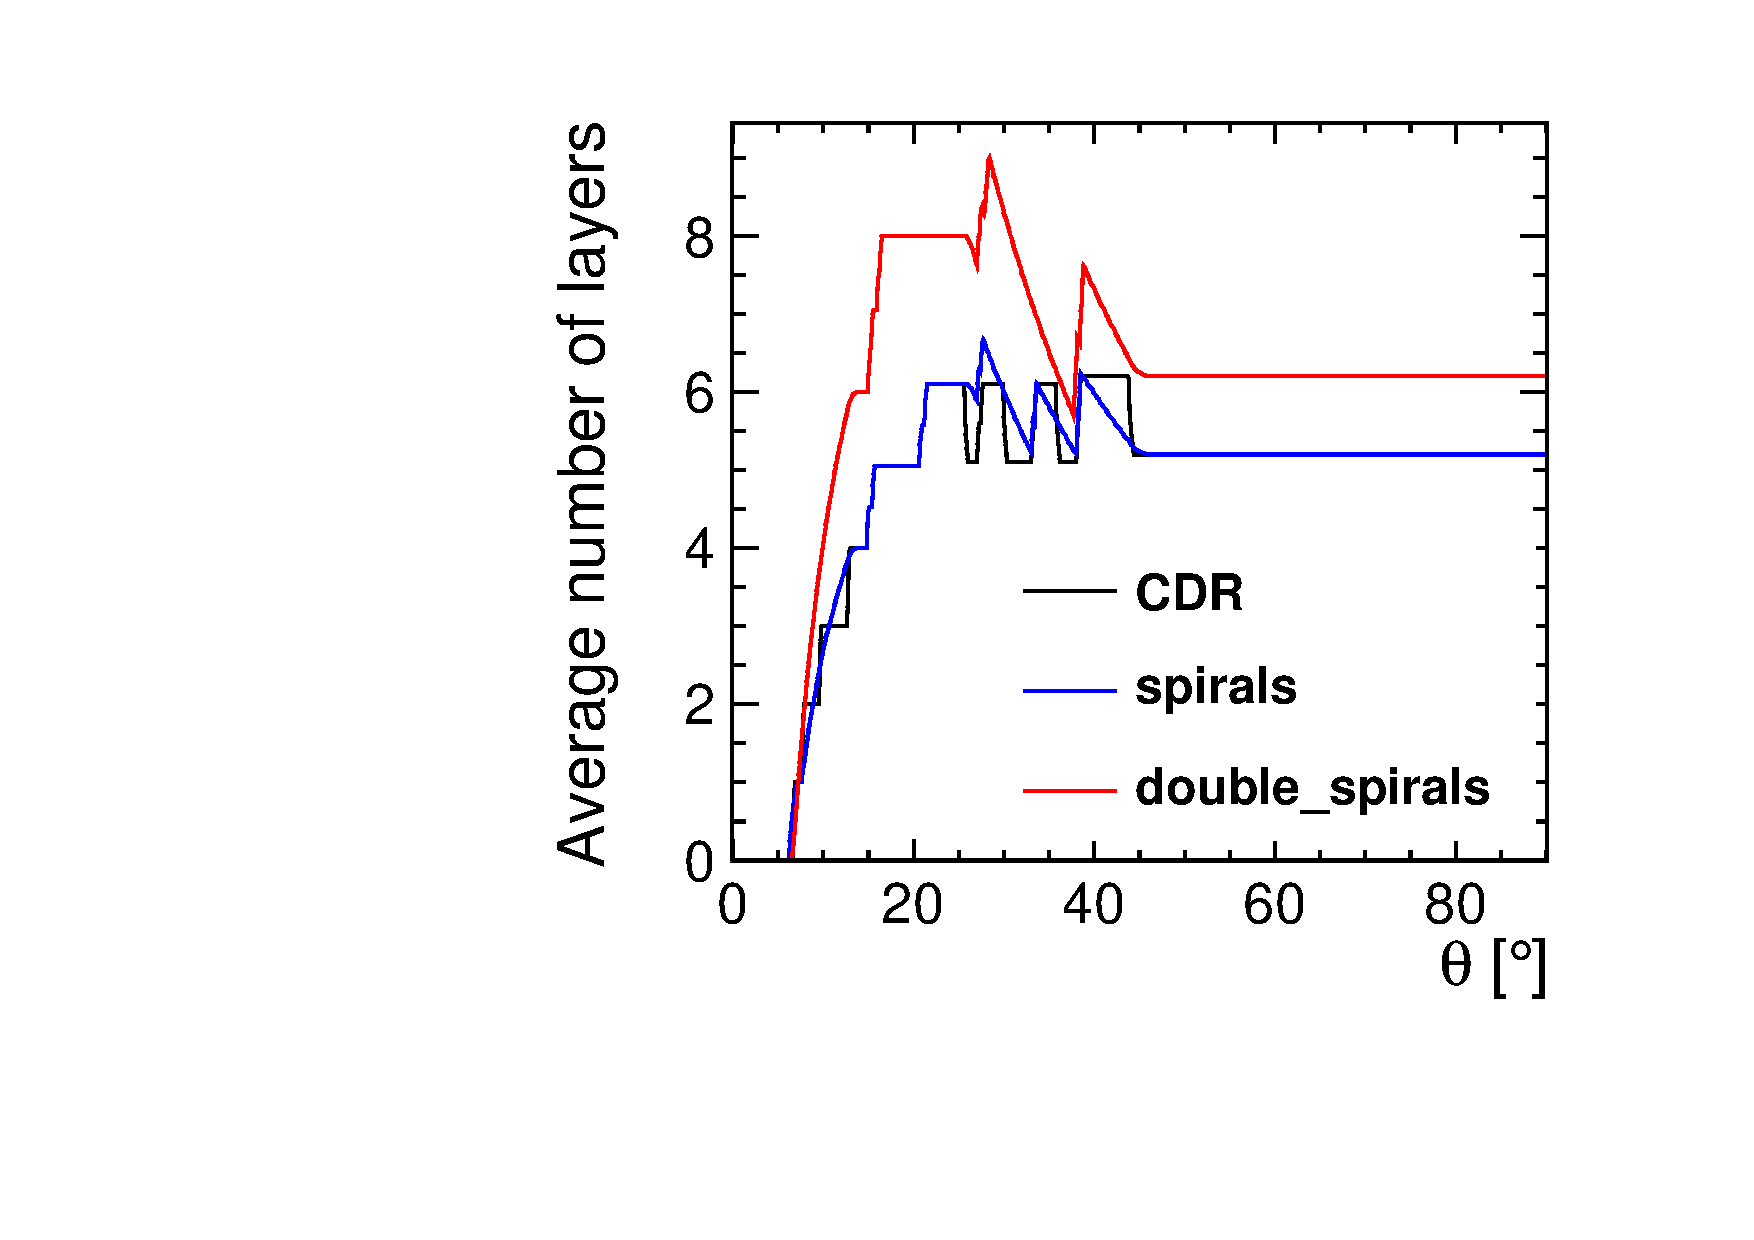
\includegraphics[scale=0.4]{Figures/Geometries/avg_nb_layers_allGeoms.pdf}
  \caption{The coverage of the vertex detector for 3 different geometries with respect to the polar angle $\theta$. The number of sensitive layers are averaged over the azimuthal angle $\phi$.}
  \label{fig:vertex_nb_layer}
\end{figure}

Figure~\ref{fig:nbLayers_theta_phi} shows the number of layers as function of the polar angle $\theta$ and the azimuthal angle $\phi$ for the \begin{it}spirals\end{it} and the \begin{it}double\_spirals\end{it} geometries in the endcap regions. For polar angles around $\theta=40^{\circ}$, the number of layers becomes very dependent on the azimuthal angle $\phi$. In this region, there is a transition between the endcaps and the barrel sections. Using a spiral arrangement of the sensors in the vertex endcaps introduces a $\phi$ asymmetry in the coverage, see Figures~\ref{fig:singleSpiralGeom} and \ref{fig:doubleSpiralGeom}.
For some discrete $\phi$ angles, the number of layers is twice the one
at neighbouring $\phi$ angles (Figure~\ref{fig:nbLayers_theta_phi}). This can be explained by the fact that for a given  $\theta$, neighboring modules have a small overlap in $\phi$.

\begin{figure}[H]
        \begin{subfigure}[b]{0.5\textwidth}
          \centering
          %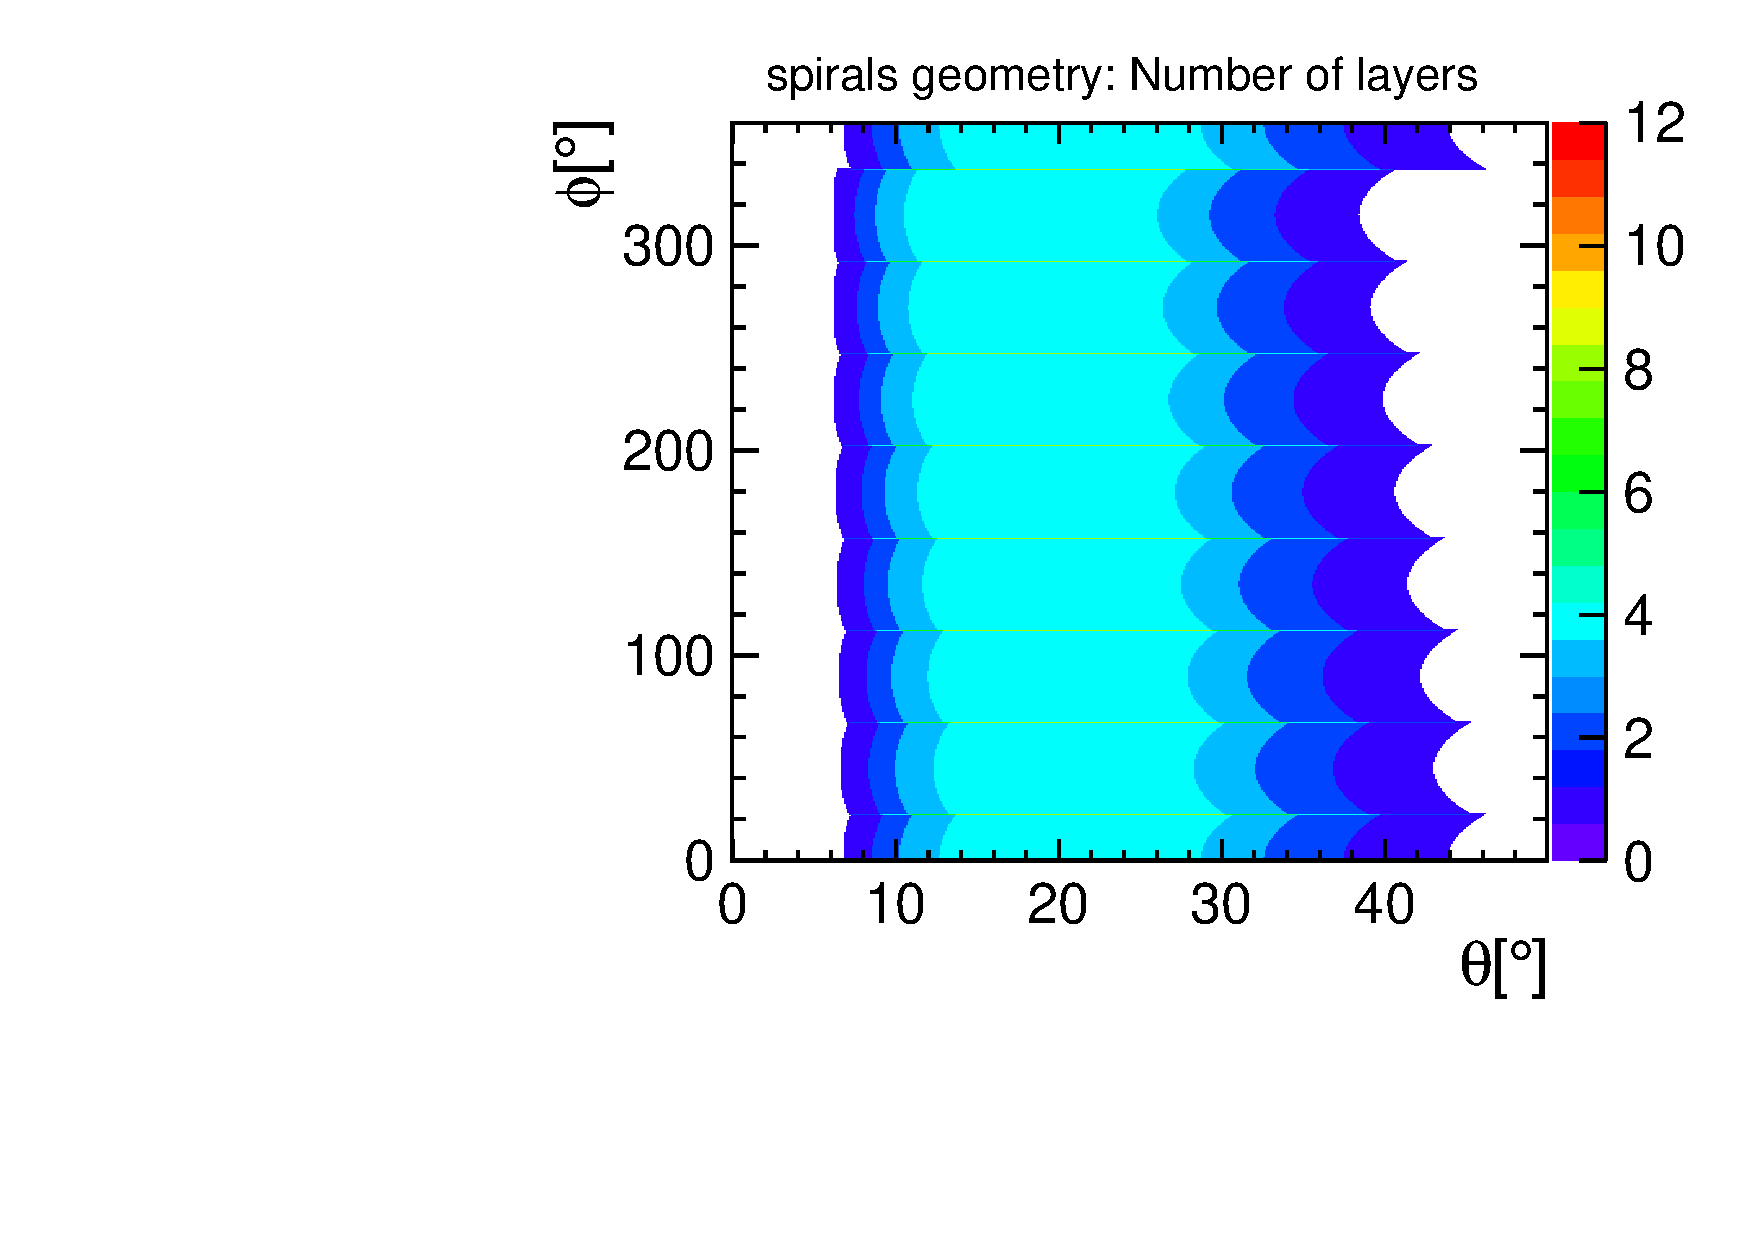
\includegraphics[width=\textwidth]{Figures/Geometries/spirals_theta_phi.pdf}
          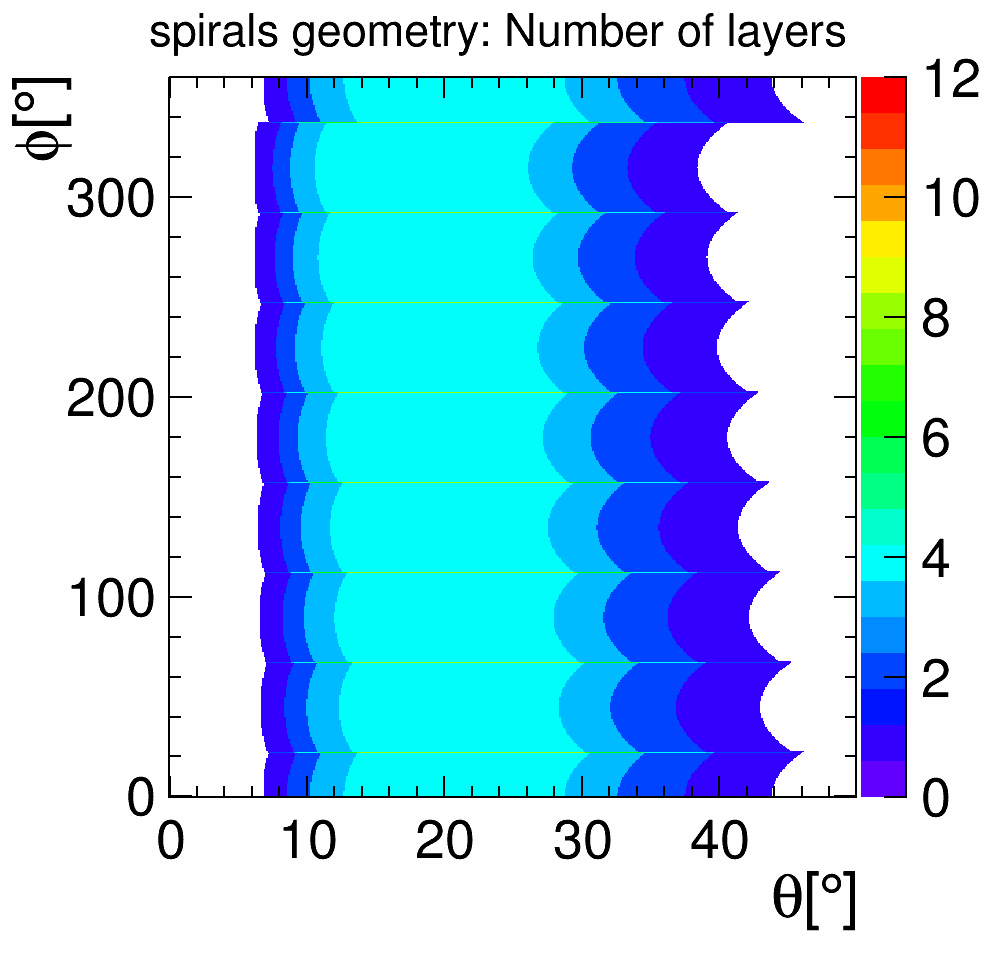
\includegraphics[width=\textwidth]{Figures/Geometries/spirals.png}
          \caption{}
          \label{}
        \end{subfigure}%
        ~ 
        \begin{subfigure}[b]{0.5\textwidth}
          \centering
          %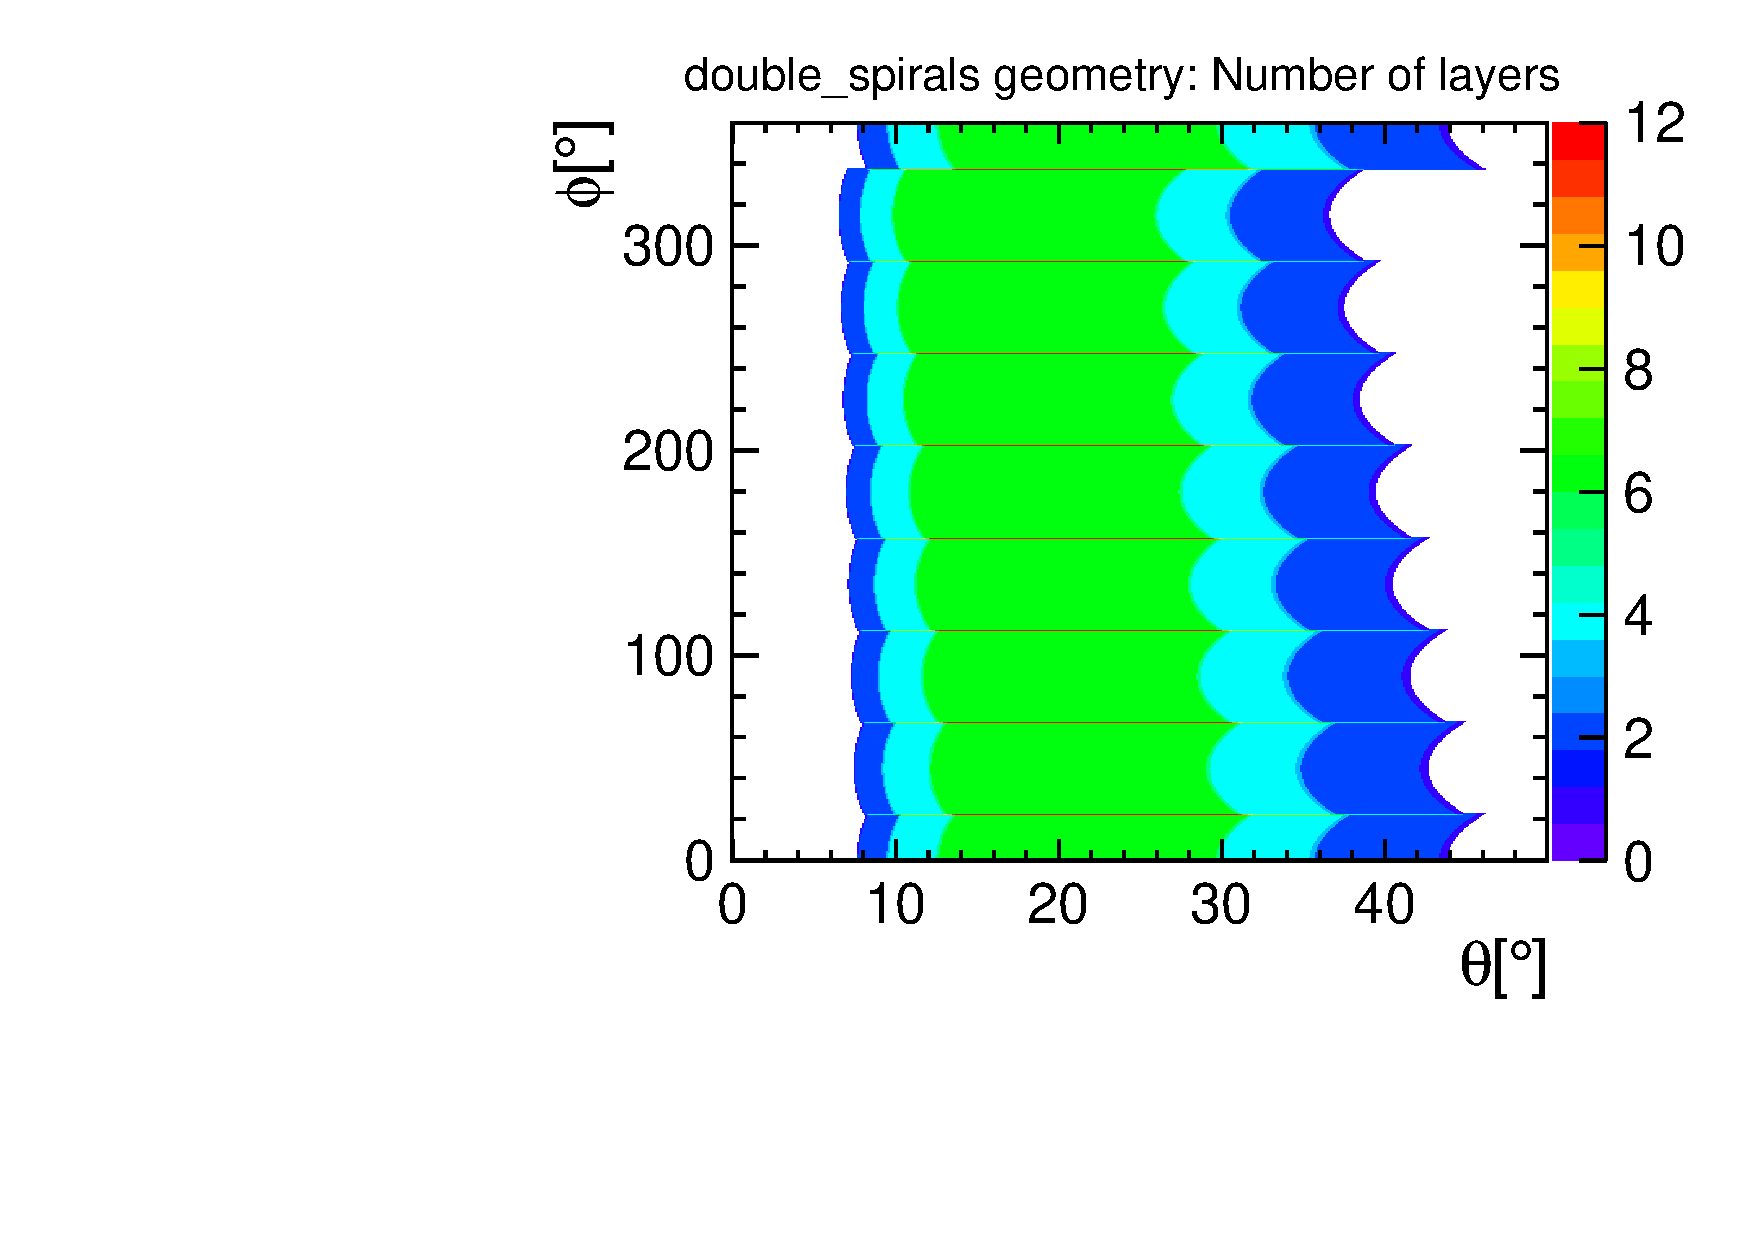
\includegraphics[width=\textwidth]{Figures/Geometries/double_spirals_theta_phi.pdf}
          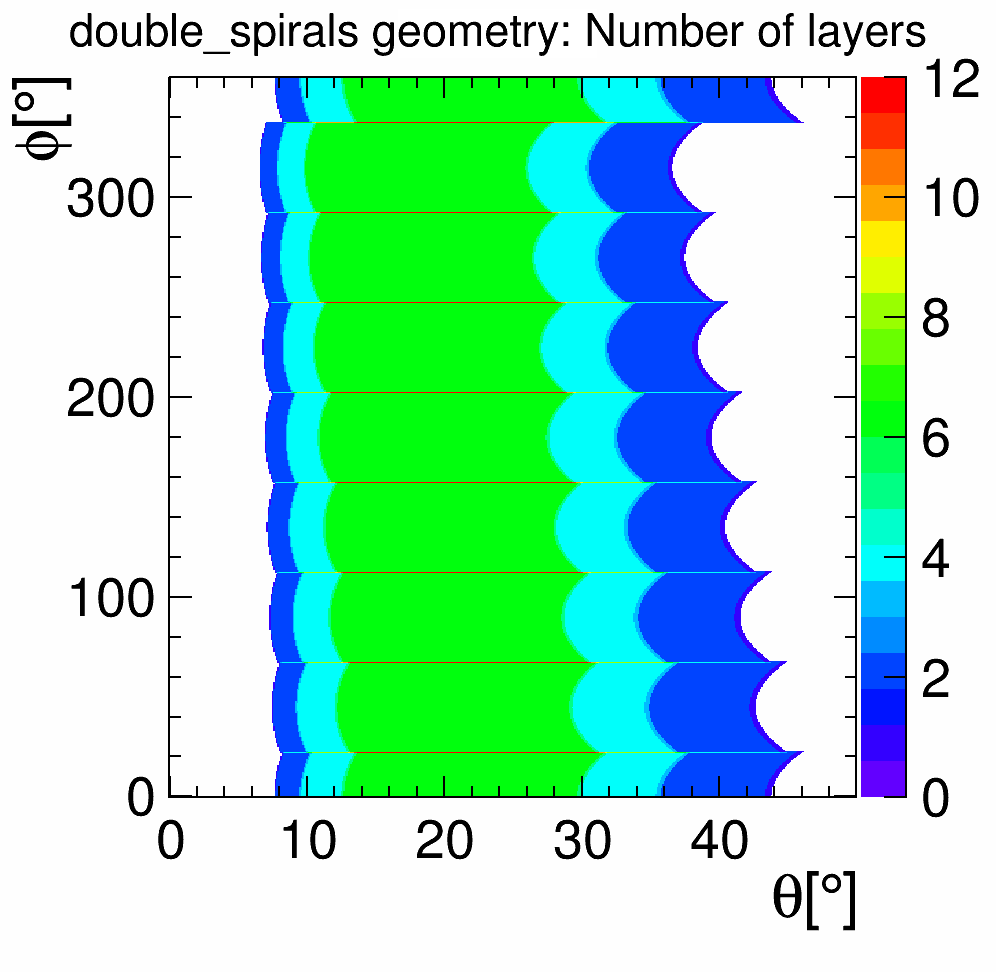
\includegraphics[width=\textwidth]{Figures/Geometries/double_spirals.png}
          \caption{}
          \label{}
        \end{subfigure}
        \caption{Number of layers as a function of the polar angle
          $\theta$ and of the azimuthal angle $\phi$ for the {\it
            spirals} and the {\it double\_spirals} geometries in the endcap regions. }\label{fig:nbLayers_theta_phi}
\end{figure}
%----------------------------------------------------------------------
\subsection{The \emph{double\_spirals\_v2} geometry}\label{sec:CLIC_SiD_double_spirals_heavy}

In engineering studies, a double-layered module is estimated to have a material budget of $0.4\%X_{0}$. This value takes into account two silicon sensors with a thickness of \SI{50}{\micro\meter}, the ASIC of \SI{50}{\micro\meter}, the carbon fiber for the mechanical support, the electronics used for the power pulsing and the cables~\cite{Blanchot:1635206}. \\
The \begin{it}double\_spirals\_v2\end{it} geometry has the same layout
as \begin{it}double\_spirals\end{it}
(cf. Section~\ref{sec:CLIC_SiD_double_spirals}), but with a material
budget of $0.4\%X_{0}$ per double layer. In the simulation, this was
achieved by modules of silicon followed by \SI{13.5}{\micro\meter} of
copper. The material budget for the \textit{double\_spirals\_v2} geometry is for example 1.6 times higher at $\theta=90^{\circ}$ than that of the CDR geometry as shown in Figure~\ref{fig:material_budget_heavy_double_spirals}.

\begin{figure}[H]
  \centering
    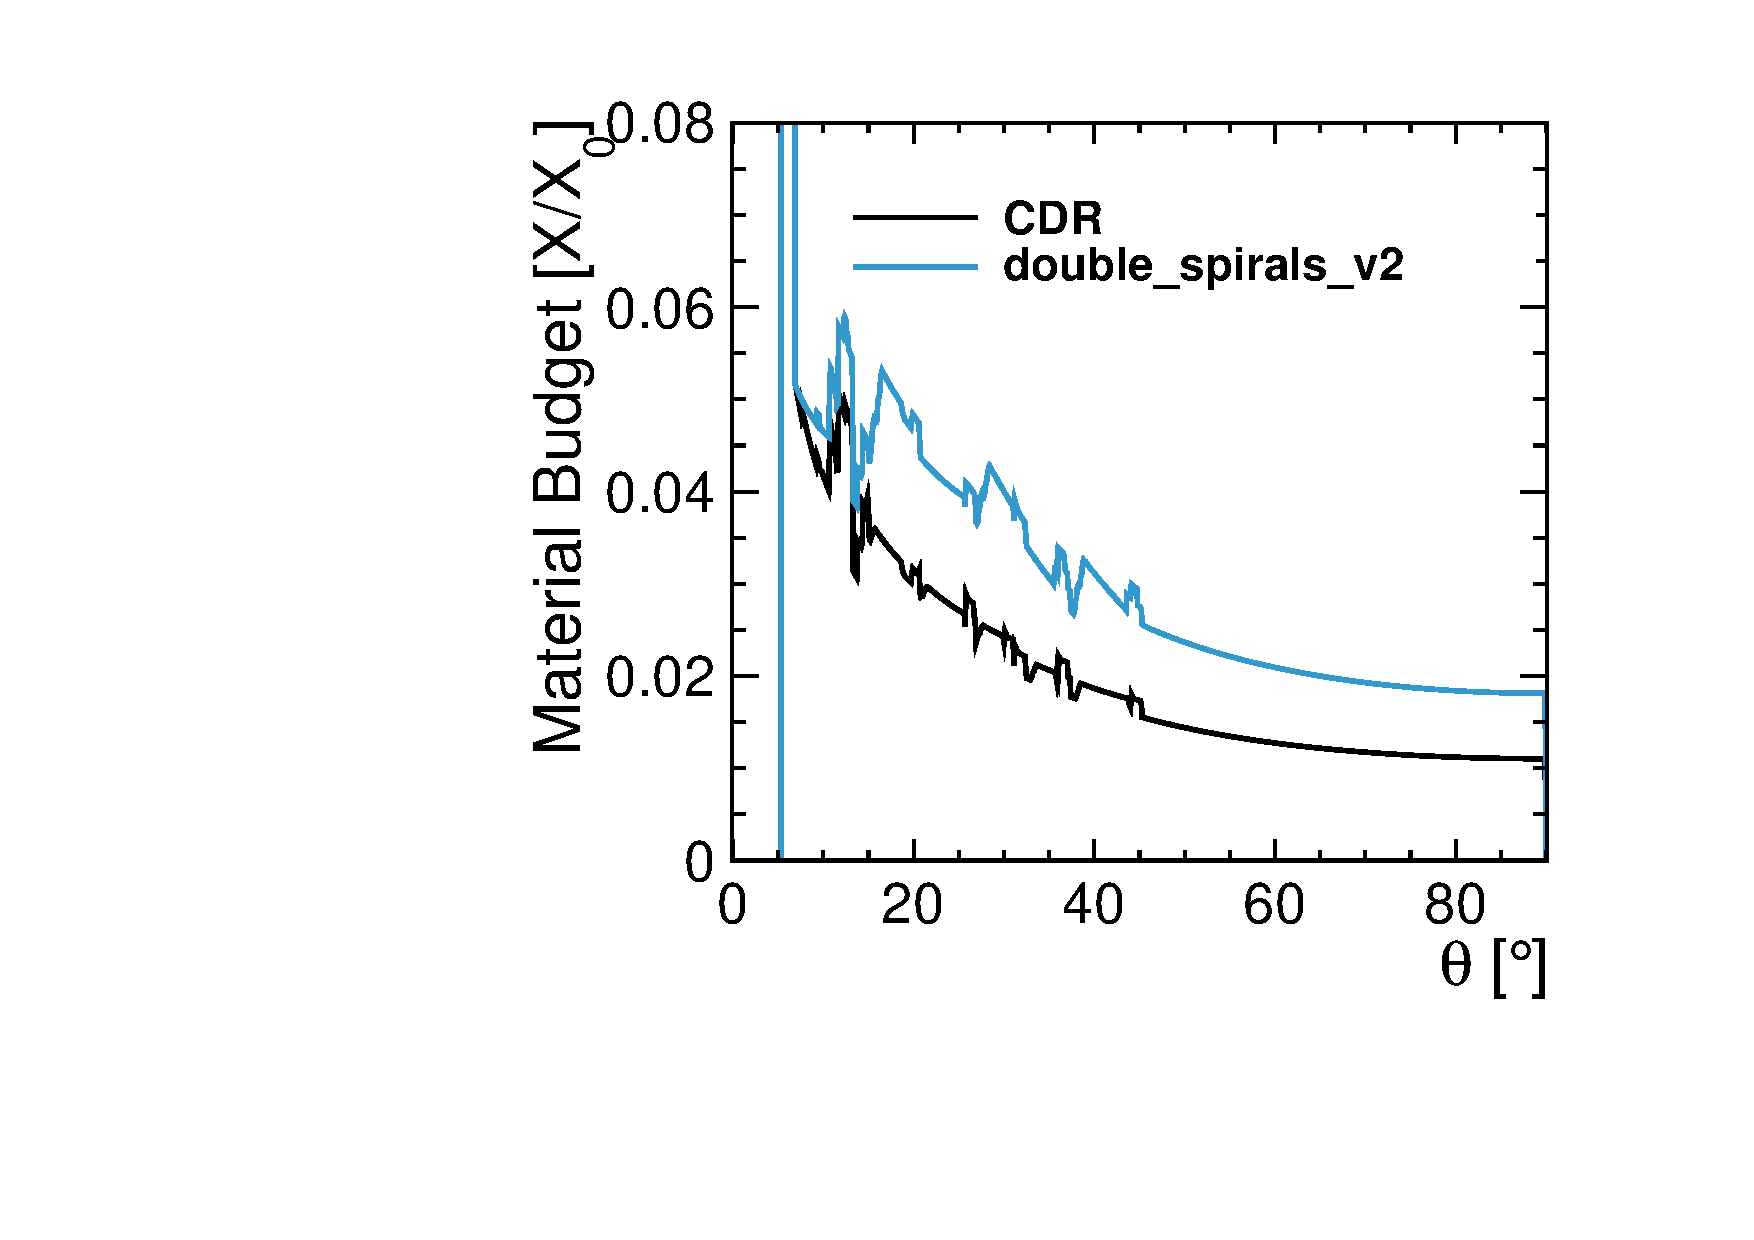
\includegraphics[scale=0.4]{Figures/Geometries/material_budget_heavy_double_spirals.pdf}
    \caption{The simulated material budget for the CDR and {\it double\_spirals\_v2} geometries. For each polar angle $\theta$, the material budget is averaged over the azimuthal angle $\phi$.}
    \label{fig:material_budget_heavy_double_spirals}
\end{figure}
